\section{Introduction}

Recent advances in small Unmanned Aircraft Systems (UAS) perception systems are beginning to enable safe three-dimensional navigation through complex uncertain environments for applications such as aerial photography, infrastructure inspection, search and rescue, and package delivery. Urban UAS operations will necessarily occur above buildings and over people. A safe urgent landing capability is a necessity, but no terrain-based or prepared vertiport landing option \cite{patterson_timely_2014, atkins_emergency_2006, di_donato_evaluating_2017} may be available.  In densely-populated urban regions, building rooftops can offer nearby safe landing zones for small UAS \cite{desaraju_vision-based_2015}. Urban roofs often have flat-like characteristics and are usually free from human presence \cite{castagno_roof_2018}. However, landing on urban buildings provides unique challenges such as avoiding auxiliary structures hosted on each rooftop.  A database of flat rooftops, their topologies, and optimal touchdown points can be computed and stored a priori from data such as satellite imagery and airborne survey point clouds \cite{castagno_map-based_2021}. However, a sUAS must identify a touchdown point on approach to an unprepared rooftop landing site to confirm the landing zone is clear or replan as needed.

\begin{figure}[!ht]
    \centering
    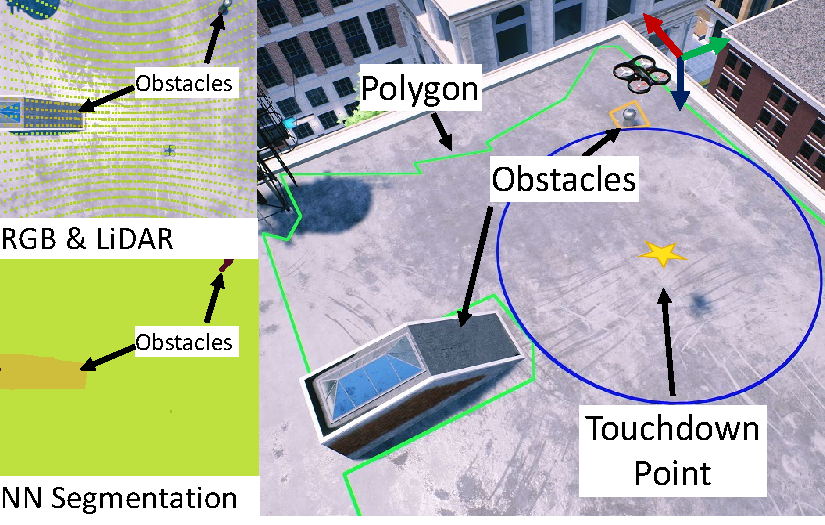
\includegraphics[width=0.70\columnwidth]{chapter_6_landingsim/figs/main_photo.pdf}
    % \includegraphics[width=0.99\columnwidth]{imgs/Overview_LS_Identification_rev2.pdf}
    \caption[Overview of Semantic Polylidar3D]{Overview of Semantic Polylidar3D for touchdown point selection. Camera RGB (red-green-blue) images are transformed into a segmented image through a neural network. LiDAR point cloud data is projected into the segmented image for classification. Flat surfaces are extracted with Semantic Polylidar3D \cite{castagno_polylidar3d_2020} from the \textit{classified} point cloud as shown in the right image indicating a green candidate landing site polygon with orange interior ``obstacle cutouts''. The blue circle represents the largest flat, obstacle-free touchdown point in the polygon.}
    \label{fig:ch6_ls_overview}
\end{figure}

This paper proposes Semantic Polylidar3D, a suite of computational geometry (Polylidar3D \cite{castagno_polylidar3d_2020}) and deep neural network (semantic segmentation  \cite{howard_mobilenets_2017, ronneberger_u-net_2015} algorithms to identify and select safe rooftop landing zones in real time using a combination of LiDAR and camera sensors.  A high-fidelity simulated city is constructed in the Unreal game engine \cite{unrealengine} with particular attention given to creating a statistically-accurate representation of rooftop obstacles that create obstructions to safe landing, e.g., water towers, vents, air conditioning units, rooftop building access doors.    AirSim \cite{shah_airsim_2018}, a robotic vehicle simulator plugin for Unreal, generates onboard small UAS video and LiDAR data feeds as the small UAS navigates through the simulated Unreal environment.  Semantic Polylidar3D fuses small UAS image and LiDAR data to compute the optimal obstacle-free touchdown circle on a rooftop within UAS sensor field of view. Figure \ref{fig:ch6_ls_overview} provides a graphical overview of processing steps. A LiDAR point cloud is classified by projecting data into a semantic image generated by a neural network. The classified point cloud is then rapidly converted into a polygon representing clear landing area accounting for both geometric and semantic information. Key contributions include:

\begin{itemize}
  \item Construction of a high-fidelity visual city model from real world data of the rooftops in midtown Manhattan, New York.
  \item A hybrid algorithm for planar extraction accounting for semantic information using computational geometry and deep learning.
  \item A novel method for finding optimal touchdown points on rooftops in a processing pipeline viable for real-time deployment. 
  \item A comparative study of state-of-the-art semantic segmentation models to show their classification accuracy.
\end{itemize}
%  rooftop and obstacle identifying 

Below, a summary of related work (Section \ref{sec:ch6_related_work}) is followed by a problem statement (Section \ref{sec:ch6_problem_statement}) and definitions (Section \ref{sec:ch6_definitions}).  Section \ref{sec:ch6_touchdown_point_selection} describes our touchdown point selection procedure using Semantic Polylidar 3D.  The urban rooftop simulation environment is presented in Section \ref{sec:ch6_simulation_environment}, and results are presented for semantic segmentation (Section \ref{sec:ch6_segmention_results}) and the integrated Semantic Polylidar3D pipeline (Section \ref{sec:ch6_touchdown_point_results}).  The paper concludes with a discussion (Section \ref{sec:ch6_discussion}) followed by a brief conclusion (Section \ref{sec:ch6_conclusions}).

\section{Related Work}\label{sec:ch6_related_work}

This section first summarizes the literature in aircraft unprepared landing site selection with focus on vertical takeoff and landing (VTOL) platforms including multicopter small UAS.  Background in image pixel classification for semantic segmentation and polygon extraction is also provided. 

\subsection{Unprepared Landing Site Selection}\label{sec:ch6_related_landing}

VTOL aircraft have been flown extensively in unmapped and dynamic environments, historically with onboard radar and vision guiding approach to landing in manned helicopter operations \cite{scherer_autonomous_2012}. Per  \cite{jin_-board_2016} and \cite{desaraju_vision-based_2015}, terrain landing sites are commonly investigated and still remain the primary alternative to runways/vertiports for VTOL aircraft.  Rooftop landings have only recently been considered \cite{desaraju_vision-based_2015, castagno_comprehensive_2018, castagno_map-based_2021} since only emerging small UAS are sufficiently lightweight to land on a roof without risking structural damage or collapse.    Regardless of touchdown site specifics, landing can be decomposed into three steps: landing site identification and selection, landing trajectory generation (flight planning), and flight plan execution \cite{atkins_emergency_2006, dotenco_autonomous_2015}. This paper is specifically focused on real-time local perception for rooftop-based landing site identification and selection.

Cameras are a common sensors used for landing site identification.  For example, Ref. \cite{jin_-board_2016} relies on monocular vision, an inexpensive lightweight option for small UAS. Monocular cameras can use structure from motion (SfM) to generate 3D point clouds of the environment to aid in scene understanding \cite{schonberger_structure--motion_2016}, but map accuracy is often limited from computational constraints.  Ref. \cite{desaraju_vision-based_2015} uses stereo vision to aid in depth mapping, while Ref. \cite{whalley2009field} uses a custom LiDAR system to avoid obstacles and identify clear/flat terrain for approach and landing.  Recently  LiDAR sensors have become sufficiently lightweight and economical to be carried onboard small UAS.  LiDAR provides precise range estimates to surfaces and can be directly transformed to 3D point clouds.  However this precision comes at a cost increase, and point clouds may experience distortion when mounted on moving vehicles such as small UAS.  Solid state LiDAR sensors with few to no moving parts reduce motion distortion, and offer corresponding reductions in weight and cost \cite{wei_enhancing_2021, nam_solid-state_2021, nxp:tja1043}.  We assume next-generation small UAS tasked with accurately navigating a complex urban landscape will carry a camera and LiDAR. 

Researchers often use predefined landing site markers and perform image feature matching to recognize the site \cite{shuo_yang_precise_2015, yang_autonomous_2014}. These algorithms use known landing site geometry patterns to robustly estimate relative state of the aircraft to guide it through a safe touchdown.  Our work is focused on unprepared rooftop landing sites where markers will not be available so site identification and final approach guidance must be performed from natural environment features. 

Ref. \cite{pluckter_precision_2020} presents methods for a return landing to the UAS' starting position in an unstructured environment. The work implements a visual teach-and-repeat method where images are recorded during take-off and serve as known control/guide points in landing.   During landing the drone localizes to these images and descends along a similar path back to its initial position. This procedure requires the drone to be above the original UAS take-off position, making it unsuitable for use in areas never before visited. 
Ref. \cite{desaraju_vision-based_2015} identifies candidate touchdown points on rooftops using a single camera to perform 3D scene reconstruction with structure from motion generating a disparity map of a rooftop.  They note variance of the disparity map along the gravity vector corresponds to the planarity of the landing surface. Smaller changes in variance correspond to flatter surfaces. With this assumption the authors apply a kernel filter across the disparity image to identify pixels that are deemed planar, normalize the resulting image between [0,1] and perform Gaussian process smoothing. This algorithm is run over a downsampled image space to select the candidate pixel having the ``flattest'' region. This procedure for candidate landing site selection guarantees a minimum distance from obstacles but does not maximize this distance, instead optimizing over planarity. 

Ref. \cite{forster_continuous_2015} identifies terrain-based candidate touchdown points in an image plane from 2D probabilistic elevation maps generated over terrain. As in \cite{desaraju_vision-based_2015}, a monocular camera using structure from motion provides depth information for each pixel. A height discrepancy filter is applied to the depth image to determine planarity, and a distance transform is applied to the image to select the flat pixel farthest away from any non-flat site (pixel). The computational complexity of the distance transform necessitates limiting the size of the map to 100X100 pixels at all altitudes.

Instead of representing surfaces as 2D discretized elevation maps one can instead extract continuous flat sections as polygons \cite{lee_indoor_2012-1}. The authors have developed Polylidar3D \cite{castagno_polylidar3d_2020}, an algorithm and accompanying open-source software for extracting flat surfaces as non-convex polygons with interior holes representing obstacles.  Polylidar3D was previously used to find rooftop landing sites from archived airborne LiDAR point clouds  \cite{castagno_map-based_2021}. This offline processing pipeline also found touchdown points on identified flat polygons that maximize distance to any edge or interior obstacle. This paper combines Polylidar3D with a deep neural network to generate a semantic map of visible features from camera images and uses fused results for real-time touchdown point selection.

\subsection{Semantic Segmentation}\label{sec:ch6_related_pixel}
% The recent image semantic segmentation work has been summarized into three categories according to \cite{siam2018comparative}. 
Semantic segmentation describes the process of associating each pixel of an image with a class label such as \emph{sky} or \emph{rooftop}.  Fully convolutional networks (FCN) were first proposed for image semantic segmentation \cite{shelhamer_fully_2017} to learn an end-to-end encoder-decoder model capable of segmentation. The encoder model is a deep CNN that extracts image features with multiple resolutions while the decoder model contains transposed convolutions (upsampling) to predict segmentations with different resolutions. U-Net \cite{ronneberger_u-net_2015} further takes advantage of high-resolution features by decoding after each encoding CNN block. SegNet \cite{badrinarayanan_segnet_2017} is an encoder-decoder model that upsamples from a feature map by storing maxpooling indices from the corresponding encoder layer. Bayesian SegNet \cite{kendall_bayesian_2017} improves this model by adding dropout layers to incorporate prediction uncertainties.

Other semantic segmentation work utilizes context-aware models such as DeepLab \cite{chen_rethinking_2017, chen_deeplab_2018} and temporal models \cite{siam_comparative_2018}. These models have relatively high weights for mobile device applications compared to FCN-based methods. This paper compares the performance of different combinations of lightweight CNN encoders and FCN-based decoders for urban rooftop image semantic segmentation. 


\subsection{Polygon Extraction from Depth Data}

Convex polygons from RGBD images have been extracted by Ref. \cite{biswas_planar_2012} and \cite{poppinga_fast_2008}.  However, convex polygons cannot represent boundary concavities or account for holes in the polygon. Ref. \cite{lee_indoor_2012-1} generated non-convex polygons from range images using region growing but ignored interior holes. Ref. \cite{trevor2013efficient} performed polygon extraction through boundary tracing of plane-segmented range images but also ignored interior holes.

Several methods can extract non-convex polygons with interior holes, e.g., \cite{edelsbrunner_shape_1983, furieri_spatialite_2017}. These methods strictly operate on 2D data requiring the 3D planar point cloud segments be projected to the best fit geometric plane to produce 2D point sets. Ref. \cite{lee_fast_2013} proposes this technique and the use of $\alpha$-shapes to extract polygons. However this method requires computationally-expensive projection and Delaunay triangulation operations making it unsuitable for real-time applications. Polylidar3D is a faster parallelized non-convex polygon extraction method that also accounts for interior holes \cite{castagno_polylidar3d_2020}.


\section{Problem Statement}\label{sec:ch6_problem_statement}

This paper investigates rooftop touchdown point selection to enable small UAS operating in urban environments to perform safe urgent landings when necessary. Figure \ref{fig:ch6_contingency_planning} illustrates logic and data flow for the rooftop contingency landing problem. This framework unifies sensor-based and map-based planning methods previously connected  in Ref. \cite{ten_harmsel_emergency_2017}.  A small UAS requiring an urgent or emergency landing must perform landing site identification and touchdown point selection to assure landing will avoid or minimize risk to people, property, and the UAS. If an observed site is safe the UAS will plan and execute a trajectory to that site. If the area is not safe the on-board map will be updated and a map-based planner will identify an alternate site. Archived map data may be used to find an alternate minimum-risk landing site that may be beyond UAS sensor field of view. On approach to this alternate site, real-time map and touchdown point confirmation will occur. The cycle will repeat as needed. 

\begin{figure}[ht!]
\centering
% 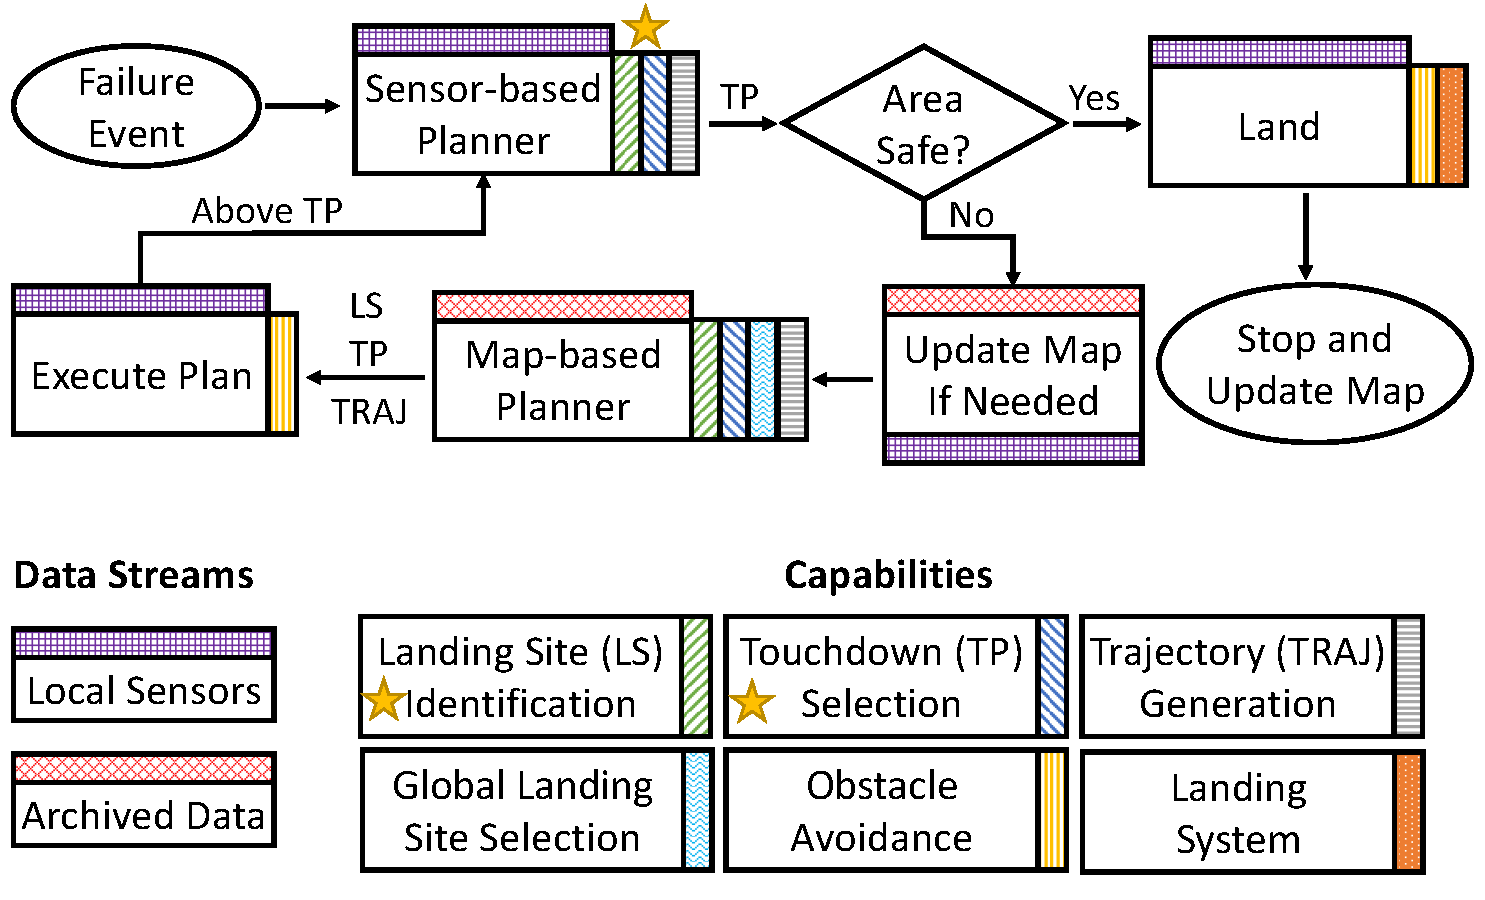
\includegraphics[width=.95\linewidth]{chapter_6_landingsim/figs/problem_statement_overview_2.pdf}
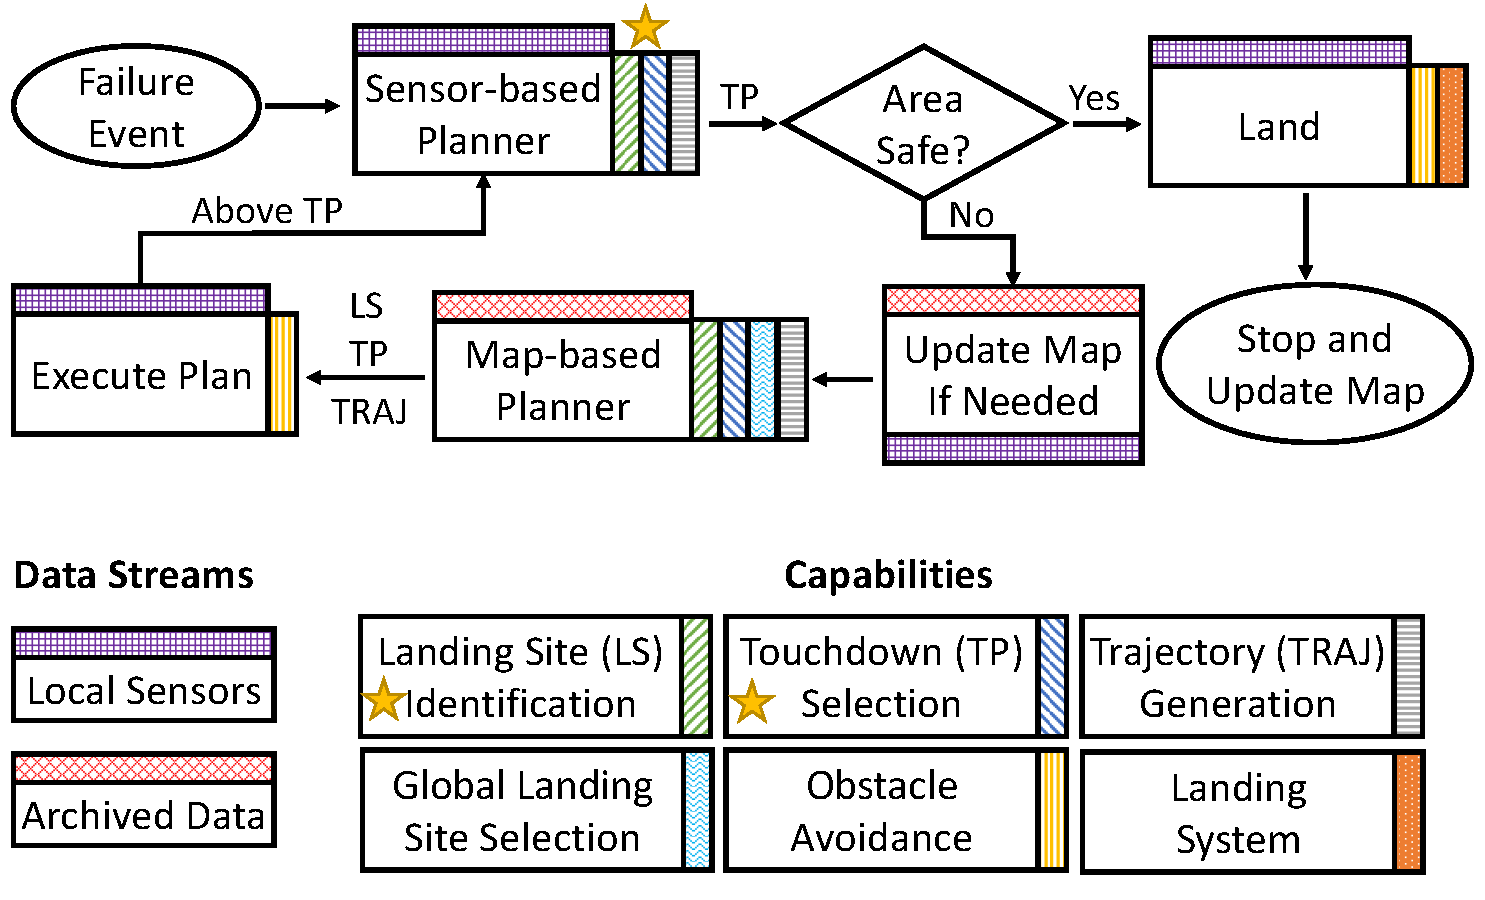
\includegraphics[width=.85\linewidth]{chapter_6_landingsim/figs/problem_statement_overview_2.pdf}
\caption[Rooftop-based contingency landing planning overview]{Rooftop-based contingency landing planning overview. Boxes with gold stars indicate research focus for this paper. }
\label{fig:ch6_contingency_planning}
\end{figure}

This paper builds on previous work in map-based planning with geographic information system (GIS) data processed offline. In earlier work, GIS satellite imagery and airborne LiDAR point clouds were used to construct a database of flat rooftops and their associated optimal touchdown points  \cite{castagno_map-based_2021}. Such a database can be loaded on the UAS before takeoff and used by a map-based planner to guide landing site selection and trajectory generation. This paper builds on previous terrain-based landing site identification summarized above (e.g., \cite{scherer_autonomous_2012}) to support complex flat rooftop sensor-based landing site confirmation and touchdown point selection using on-board LiDAR and camera sensors.

This work assumes the small UAS is equipped with a LiDAR sensor and monocular camera mounted underneath the vehicle. The small UAS also must carry a computer sufficient for sensor data processing and fusion. This work assumes the UAS has previously selected a rooftop landing site from onboard maps and that the UAS has executed an approach trajectory to a hover waypoint ten meters above the mapped touchdown point. This paper proposes a process to integrate visual (camera) and depth (LiDAR) data streams to verify the landing site is safe (e.g., flat and clear) and adjust the touchdown point if needed. If a safe touchdown point is found a controlled landing will then be executed; otherwise the UAS must fly to an alternate mapped landing site.  By converting depth data to planar surfaces and video data to surface type with semantic segmentation, the UAS can conform/identify a clear and suitable touchdown point in real-time. Because a number of semantic segmentation methods have been developed, comparative benchmarking over realistic datasets is required to quantitatively assess options.  This paper relies on simulation-based datasets designed to be statistically similar to rooftops in Manhattan since we cannot reasonably fly small UAS above Manhattan buildings to collect actual flight data.

\section{Definitions}\label{sec:ch6_definitions}

A scanning LiDAR that completes a full revolution generates a range image. This image has $M$ rows denoting the number of beams in the vertical direction and $N$ columns each representing a laser return in the full sequential scan. The range image can be converted to an organized 3D point cloud $\mathcal{P}$. 

% This organized point cloud is structured with 2D indices $u \in [0, M -1], v \in [1, N -1]$ such that $\vec{p}_{u,v} = [\vec{x}_{u,v}, \vec{y}_{u,v}, \vec{z}_{u,v}]$.   Neighboring 2D indices ($u,v$) and ($u+1, v+1$) represent 3D proximity relationships between $p_{u,v}$ and $p_{u+1,v+1}$ when they lie on the same surface. 

A \textit{linear ring} is a consecutive list of points that is both closed and simple \cite{herring_opengis_2006-1}. A linear ring must have non-intersecting line segments that join to form a closed path. A valid \textit{polygon} has a single exterior linear ring representing the shell of the polygon and a set of linear rings (possibly empty) representing holes inside the polygon. The vertices of the polygon may be 3D points assuming all points lie on a 2D plane.

Figure \ref{fig:ch6_frames} shows the reference frames defining vehicle body, camera, and LiDAR sensor placements and orientations.  Vehicle body frame \{B\} has $x$-axis pointing forward, $z$ axis pointing down, and $y$-axis completing a right-hand orthogonal frame. Camera frame \{C\} and LiDAR \{L\} have a translation offset of $\begin{pmatrix}-0.05 & 0 & -0.05\end{pmatrix}$ and $\begin{pmatrix}0.05 & 0 & -0.05\end{pmatrix}$ respectively in the body frame. LiDAR frame \{L\} follows the same conventions as body frame except rotated $90^\circ$ about body $y$ such that the LiDAR $x$ axis points directly down (aligned with body $z$). These axes conventions are the standard reference designs provided by the AirSim plugin used for simulation-based tests. The reference frame of data will be indicated by a superscript, e.g., $\mathcal{P}^{L}$ denotes a point cloud in the LiDAR frame. A homogeneous transformation from frame $A$ to frame $B$ is denoted $\mathbf{H}^A_B$.

\begin{figure}[ht]
 \centering
  \begin{subfigure}{.29\columnwidth}
    \centering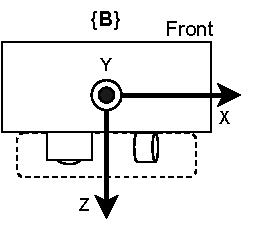
\includegraphics[clip,trim=0cm 0.30cm 0.25cm 0cm, width=.99\columnwidth]{chapter_6_landingsim/figs/Frames-FramesA.pdf}
    \caption{\label{fig:ch6_frames_a}}
  \end{subfigure}
  \begin{subfigure}{.50\columnwidth}
    \centering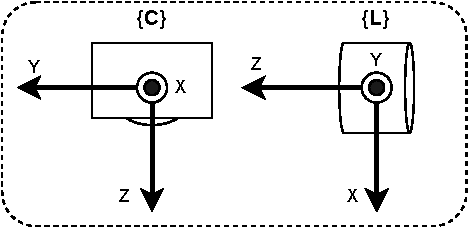
\includegraphics[page=1, width=.99\columnwidth]{chapter_6_landingsim/figs/Frames-FramesB-v2.pdf}
    \caption{\label{fig:ch6_frames_b}}
  \end{subfigure}
  \caption[Coordinate frames for sensor package]{Reference frames from a side view. (\subref{fig:ch6_frames_a}) UAS body frame \{B\}. (\subref{fig:ch6_frames_b}) Camera \{C\} and LiDAR  \{L\} frames.}\label{fig:ch6_frames}
\end{figure}

\section{Touchdown Point Selection}\label{sec:ch6_touchdown_point_selection}

Our proposed real-time touchdown point selection strategy is a hybrid algorithm with computer vision and computational geometry functions. Sec. \ref{sec:ch6_methods_semantic_segmentation} details the computer vision models used for scene understanding while Sec. \ref{sec:ch6_methods_semantic_polygons} discusses joining this information using polygon extraction. Finally, Sec. \ref{sec:ch6_methods_contingency_planning} details contingency planning steps used to identify landing sites.


\subsection{Semantic Segmentation for Scene Understanding}\label{sec:ch6_methods_semantic_segmentation}

Deep neural networks for computer vision can now accurately extract image features and segment images into semantic classes. Most semantic segmentation neural networks consist of two modules: convolutional neural network (CNN) backbones and meta-architecture elements.
CNN backbones are feature extractors or encoder networks that downsample input images to obtain high-dimensional features. This paper compares the performance of two backbone CNN networks: MobileNets~\cite{howard_mobilenets_2017} and ShuffleNet~\cite{zhang_shufflenet_2018}. MobileNets are lightweight deep networks designed for mobile devices. A standard convolution operation is factorized into a depth convolution and a pointwise convolution, termed depthwise separable convolution. ShuffleNet generalizes depthwise separable convolution and group convolution to achieve an efficient CNN encoder for a mobile device. A channel shuffle operation is applied to realize the connectivity between the input and output of different grouped convolutions.
%The original CNN block used by standard deep CNN models is replaces by a ShuffleNet unit which consists of depthwise convolution and two pointwise group concolutions. 

Meta-architectures are upsampling or decoder networks that reconstruct a segmentation image from downsampled feature maps. This paper compares two meta-architectures based on \cite{siam_comparative_2018}: FCN~\cite{shelhamer_fully_2017} and U-Net~\cite{ronneberger_u-net_2015}. FCN combines CNN features from different depths of the encoder network during upsampling to utilize the information from a higher resolution image. The FCN model applied in this paper combines feature maps from \textit{pool3, pool4} and \textit{conv7} layers to achieve better precision, known in FCN as stride 8 or FCN8s. U-Net takes advantage of the higher resolution feature by upsampling from each stage of the CNN encoder. At the end of each CNN block, the feature map is both input to the next CNN block and combined with the upsampled feature map.  Upsampling continues until a final segmentation map is created.
Our work implements and evaluates different image semantic segmentation models \cite{siam_comparative_2018} on a desktop platform with an RTX 2080 graphics processor.

\subsection{Semantic Polygon Extraction}\label{sec:ch6_methods_semantic_polygons}

The authors have previously created a computational geometry algorithm, Polylidar3D, that extracts flat surfaces as polygons  \cite{castagno_polylidar3d_2020}. Polylidar3D transforms organized point clouds into meshes and then extracts planar segments. Planar segmentation is a region growing process where a seed triangle is chosen and edge-connected triangles are expanded based solely on planarity constraints. Polygon extraction is then performed for each planar segment. This paper introduces extensions to utilize semantic information during the region growing process; we refer to this upgraded package as Semantic Polylidar3D. The process has three steps:

\begin{enumerate}
    \item Classify Points: The LiDAR point cloud is projected into a semantic image specifying the class of each pixel.
    \item Semantic Polylidar3D: Polygons are extracted from rooftops utilizing both geometric and semantic data.
    \item Touchdown Site:  The largest inscribed circle containing only viable landing polygons is defined.
\end{enumerate}

\subsubsection{Classify Points}
Each point in organized point cloud $\mathcal{P}^L$ is transformed to the camera frame and subsequently projected to the semantic image per

\begin{equation}
 \label{eq:transform_points} 
    p^{C} = \mathbf{H}^L_C \cdot p^{L} \\
    \ \ u = f_{x} \frac{x^{C}}{z^{C}}+c_{x} \\
    \ \ v = f_{y} \frac{y^{C}}{z^{C}}+c_{y}  
\end{equation}
where $p^{L} = (x,y,z,1)^T$ is a point in the LiDAR frame, $ \mathbf{H}^L_C$ is the transformation matrix, ($f_x$, $f_y$) are camera focal length values, ($c_x$, $c_y$) are camera principle point offsets, and $(u,v)$ are camera pixel coordinates.  The pixel position allows each point to have a class assignment from the semantic image. Some projected points may be outside the camera image and are classified as an ``unknown'' class, e.g. $u,v$ $<$ 0. Class assignments are stored in auxiliary data structure $\mathcal{C}$ of length $\mathcal{P}^L$.

\subsubsection{Semantic Polylidar3D} \label{sec:ch6_methods_semantic_polylidar3d}

Classified organized point cloud $\mathcal{P}^L$ is rapidly transformed into a half-edge triangular mesh $\mathcal{T}$  per \cite{castagno_polylidar3d_2020}. The vertices of this mesh have corresponding classifications from $\mathcal{C}$. Fig. \ref{fig:ch6_semantic_pl3d_a} shows these colorized classifications where green, orange, and blue denote rooftop, obstacle, and unknown classes, respectively. The plane normal of the rooftop, $\hat{n}_r$, is estimated using a Gaussian Accumulator\cite{castagno_polylidar3d_2020} and shown as a red arrow in Fig. \ref{fig:ch6_semantic_pl3d_a}. Mesh triangles are then filtered by geometric and semantic constraints per Algorithm \ref{alg:triangle_filtering}. The algorithm first loops over all triangles and calculates each triangle's maximum edge length ($l_t$), angle between its normal and the roof normal ($\theta_t$), and number of vertices in the rooftop and unknown class (lines 4-7). If the sum of rooftop and unknown vertices matches or exceeds $vert_{min}$ then semantic constraints pass (line 8). Next, the algorithm dynamically reduces the angular geometric constraint if the triangle belongs to the rooftop class (lines 9-12). This means a high confidence in semantic information may reduce the confidence threshold requirements for planarity, allowing slightly more noisy data to pass geometric constraints shown in line 13. Finally both constraints must pass for the triangle to be included in the filtered triangle set $\mathcal{T}_f$ shown as shaded blue triangles in Fig \ref{fig:ch6_semantic_pl3d_a}. A polygon is then extracted from the planar mesh segment using methods from \cite{castagno_polylidar3d_2020}.

\begin{figure}[ht]
 \centering
 \begin{subfigure}[t]{.45\linewidth}
%   \begin{subfigure}[t]{.60\linewidth}
    \centering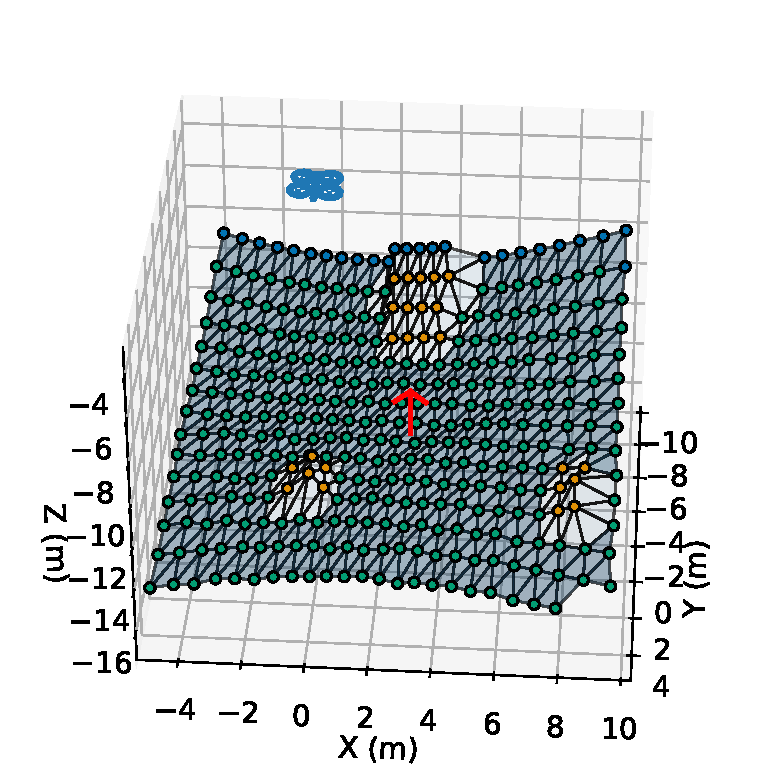
\includegraphics[clip, trim=0cm 0cm 1.25cm 0.5cm, width=.99\linewidth]{chapter_6_landingsim/figs/Algorithm_mesh.pdf}
    \caption{\label{fig:ch6_semantic_pl3d_a}}
  \end{subfigure}
  \begin{subfigure}[t]{.34\linewidth}
%   \begin{subfigure}[t]{.38\linewidth}
    \centering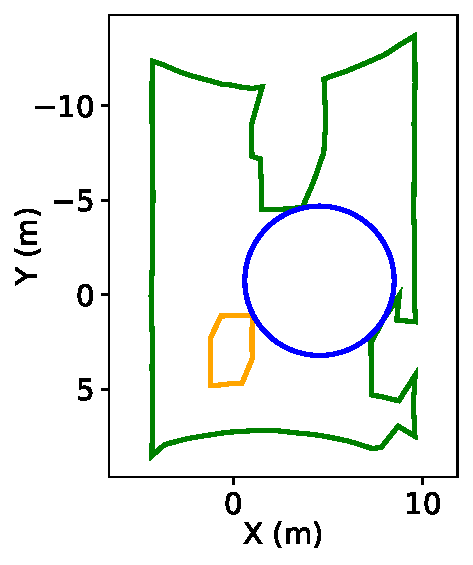
\includegraphics[page=1, width=.99\linewidth]{chapter_6_landingsim/figs/Algorithm_polygon.pdf}
    \caption{\label{fig:ch6_semantic_pl3d_b}}
  \end{subfigure}
  \caption[Visualization of Semantic Polylidar3D algorithm]{Visualization of Semantic Polylidar3D. (\subref{fig:ch6_semantic_pl3d_a}) Classified LiDAR point cloud with triangular mesh: green is rooftop, orange is obstacles, blue is unknown. Triangles meeting semantic and planarity constraints are shaded light blue. (\subref{fig:ch6_semantic_pl3d_b}) Polygon extraction from planar mesh. Green is hull, orange are interior holes, and blue is the touchdown site.}\label{fig:ch6_semantic_pl3d}
\end{figure}

\begin{algorithm}[ht]

    \SetKwInOut{Input}{Input}
    \SetKwInOut{Output}{Output}
    \SetStartEndCondition{ }{}{}%
    \SetKwProg{Fn}{def}{\string:}{}
    \DontPrintSemicolon
    % \SetKwFunction{Range}{range}%%
    \SetKw{KwIs}{is}{}
    \SetKwIF{If}{ElseIf}{Else}{if}{:}{elif}{else:}{}%
    \SetKw{KwContinue}{continue}{}
    % \AlgoDontDisplayBlockMarkers\SetAlgoNoEnd\SetAlgoNoLine%

    \Input{Triangles: $\mathcal{T}$, Points: $\mathcal{P}^L$, Class: $\mathcal{C}$, Rooftop Normal: $\hat{n}_r$ \\
           Geometric Constraint Parameters: $l_{max}, \theta_{min}, \theta_{max}$ \\
           Semantic Constraint Parameters: $c_r, c_{uk}, vert_{min}$
           }
    \Output{Filtered Triangle Set, $\mathcal{T}_f$}
    
    
    $k = |\mathcal{T}|$ \\
    $\mathcal{T}_f = \emptyset$ \\
    \tcc{Loop through every triangle}       
    \For{$t \leftarrow 0$ \KwTo  $k$ \hspace{.1cm} }{
        $l_t$ = $\operatorname{GetMaxTriangleLength}(t, \mathcal{T}, \mathcal{P})$ \\
        $\theta_t$ = $\operatorname{arccos}(\hat{n}_t \cdot \hat{n}_r$) \tcc*{triangle and roof} 
        $vert_{r}$ = $\operatorname{CountVertices}(\mathcal{C}, c_r, t)$ \\
        $vert_{uk}$ = $\operatorname{CountVertices}(\mathcal{C}, c_{uk}, t)$ \\

        \tcc{Check Semantic Constraint}  
        \texttt{semantic\_pass} = $vert_{r}$ + $vert_{uk}$ $>= vert_{min}$  \\
        
        
        \tcc{Update Angular Geometric Constraint}
        \uIf{ $vert_{r}$ $>= vert_{min}$}{
            $\theta_{req} = \theta_{max}$
        }
        \uElse{
            $\theta_{req} = \theta_{min}$
        }
        \tcc{Check Geometric Constraint}  
        \texttt{geometric\_pass} = $l_t>= l_{max}$ {\bf and} $\theta_t < \theta_{req}$  \\
        
        \tcc{Must pass both constraints}  
        \uIf{\texttt{semantic\_pass {\bf and} \texttt{geometric\_pass}}}{
           $\mathcal{T}_f$ = $\mathcal{T}_f$ + $t$
        }

    }
    return $\mathcal{T}_f$
    \caption[Semantic Triangle Filtering]{Semantic Triangle Filtering}
    \label{alg:triangle_filtering}
\end{algorithm}

\subsubsection{Touchdown Site}

Several polygons representing disjoint flat surfaces may be returned from Sec. \ref{sec:ch6_methods_semantic_polylidar3d}. These polygons may be filtered by area size, shape complexity, or even distance from the UAS. Currently the polygon with the largest area that is nearest to the drone is selected. The candidate touchdown site is determined by finding the center of the largest inscribed circle in the polygon. The largest inscribed circle in the polygon maximizes the distance between the exterior hull and any obstacles within the polygon \cite{castagno_map-based_2021, garcia-castellanos_poles_2007}. We use the software polylabel to perform this function \cite{noauthor_github_2018-3}. Fig. \ref{fig:ch6_semantic_pl3d_b} shows the greatest inscribed circle (blue) inside the polygon. A touchdown site is considered safe if it meets an aircraft-specific minimum radius constraint for safe landing clearance. If no safe touchdown site can be found then contingency planning to a new site must be performed as described below.

\subsection{Contingency Planning Overview}\label{sec:ch6_methods_contingency_planning}

If no touchdown site can be found at the initial UAS-approached rooftop then the UAS must land elsewhere and updates to inaccurate map data of that rooftop can be proposed. This may occur because of structural changes, temporary objects being placed on the surface, or dynamic obstacles (e.g., people) being present. Control authority must then switch from the sensor-based planner to the map-based planner as shown in Figure \ref{fig:ch6_contingency_planning}. The map-based planner will then select a new landing site and touchdown point that optimizes both travel distance and landing site suitability \cite{castagno_map-based_2021}. The process then repeats with the sensor-based planner verifying the landing site during each approach.

\section{Simulation Environment}\label{sec:ch6_simulation_environment}

\subsection{Analysis of Rooftops}\label{sec:ch6_rooftop_analysis}

Before constructing the simulation environment, an analysis of rooftops in Manhattan was performed. Since our work is focused on flat rooftop landing sites, only flat-like roofs in Manhattan were sampled. Data was collected manually by inspecting high resolution satellite and aerial imagery of buildings and recording the rooftop assets and associated quantities observed. Figure \ref{fig:ch6_ny_rooftops} shows the locations of 112 buildings randomly chosen from Manhattan near the Southwest corner of Central Park. The  data are released in  \cite{Castagno_Github_UnrealLanding}.

\begin{figure}[ht!]
\centering
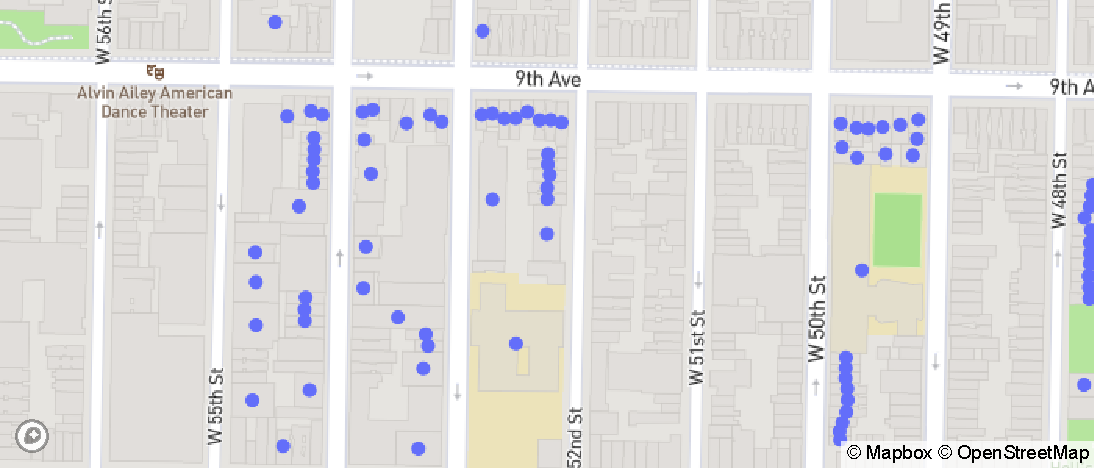
\includegraphics[angle=0,origin=c,width=.75\columnwidth]{chapter_6_landingsim/figs/map_ny_vector.pdf}
\caption[Map of Manhattan buildings observed for rooftop assets]{Map of Manhattan buildings. Each blue circle represents a rooftop  used for asset analysis.}
\label{fig:ch6_ny_rooftops}
\end{figure}

Table \ref{table:roof_quantity} lists the 12 most common object types found on a building rooftop in midtown Manhattan and the average quantity observed. If a building does not contain an asset its quantity is recorded as zero.  The full histogram of rooftop assets is shown in Figure \ref{fig:ch6_histogram_sampling} with a logarithmic vertical axis scale.

\begin{table}[ht]
\centering
\caption{Common rooftop items with average quantities.}
\label{table:roof_quantity}
\begin{tabular}{@{}lc@{}}
\toprule
Item                   & Mean Quantity \\ \midrule
air-vents              & 1.12          \\
small-rooftop-entrance & 0.88          \\
skylight               & 0.51          \\
small-building         & 0.45          \\
ac-unit                & 0.28          \\
seating                & 0.12          \\
air-ducts              & 0.11          \\
water-tower            & 0.10          \\
chimney                & 0.05          \\
enclosed-water-tower   & 0.04          \\
tarp                   & 0.03          \\
vegetation             & 0.02          \\ \bottomrule
\end{tabular}
\end{table}

\begin{figure}[ht!]
\centering
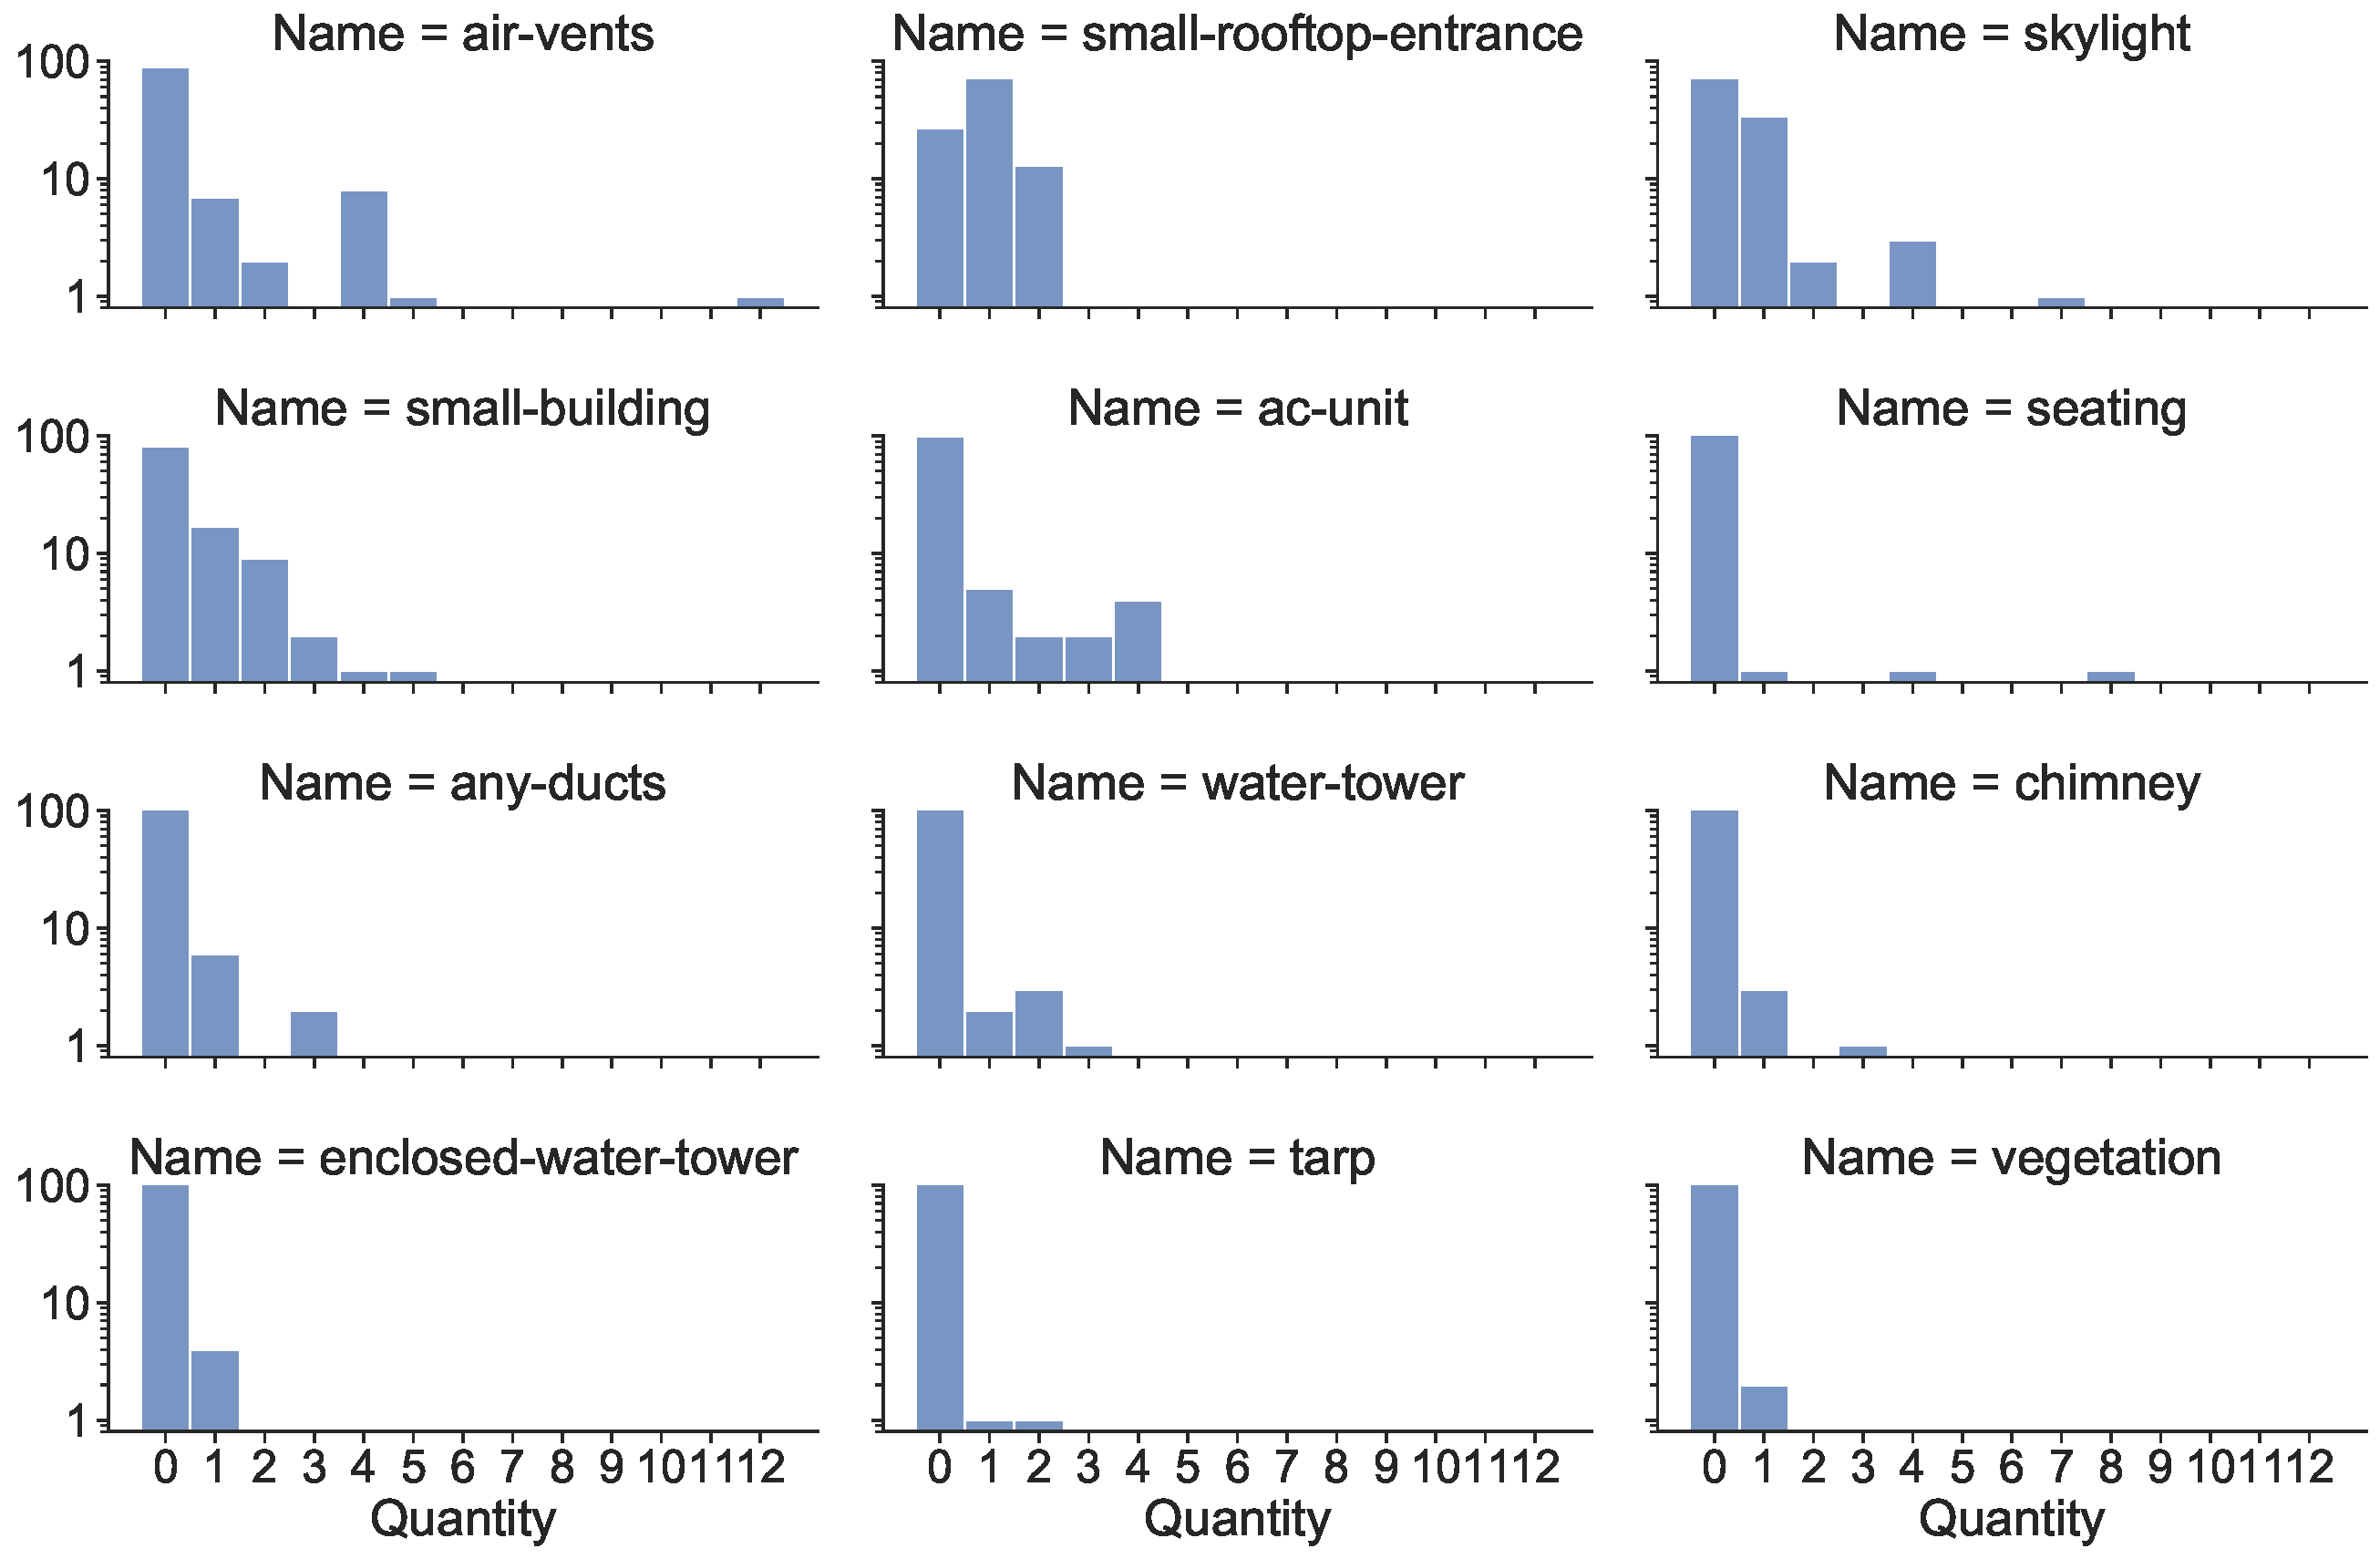
\includegraphics[width=.80\linewidth]{chapter_6_landingsim/figs/hist.pdf}
\caption[Histogram of twelve common rooftop items observed from a Manhattan dataset]{Histogram of twelve common rooftop items observed from a Manhattan dataset. }
% Two different sampling techniques are shown, directly sampling from a histogram (orange) and sampling from a fitted kernel density estimator (blue)
\label{fig:ch6_histogram_sampling}
\end{figure}


\subsection{Generating City Rooftop Environments}

Game assets for urban city buildings were purchased from \cite{urbancity}, and high quality rooftop assets (e.g., ac-units, water towers) were purchased from \cite{urbanrooftop}. Assets were modified to support configurability in textures and material properties to enhance world diversification. For example, an air-vent can be configured to take on a variety of different metal textures and reflectivity properties. Figure \ref{fig:ch6_all_assets} shows a small sample of the diversity in asset classes. A base city was constructed with 33 buildings having different building textures, sizes, and shapes. This base city served as a starting template to generate random worlds per a world generation script described below. These worlds served as the basis for training and testing purposes. Note that for this work diversity is focused on building rooftop assets, not the buildings themselves. 

A map of the base world colorized by height is shown in Figure \ref{fig:ch6_map_base_a}. Each polygon represents the flat surface of a rooftop with known height. A world generation script takes as input this map as well as an asset configuration file and places assets on each rooftop in a new 3D world. This script supports configurable options including: probability and quantity of asset placement, spatial location on the rooftop, asset orientation, and appearance properties (e.g. materials, textures, meshes).  The distribution curve for new asset placement is assumed independent of assets already placed on a building for simplicity. The quantity of assets can either be configured to follow a uniform distribution or model the histogram shown in Figure \ref{fig:ch6_histogram_sampling}. Each world is seeded with a different number to create diverse and reproducible worlds. Figure \ref{fig:ch6_map_base_b} shows an example of building assets being placed randomly on a roof per the world generation script. The  world generation script is released with this manuscript and may be used in any Unreal Engine project \cite{Castagno_Github_UnrealLanding}.


\begin{figure}[ht!]
\centering
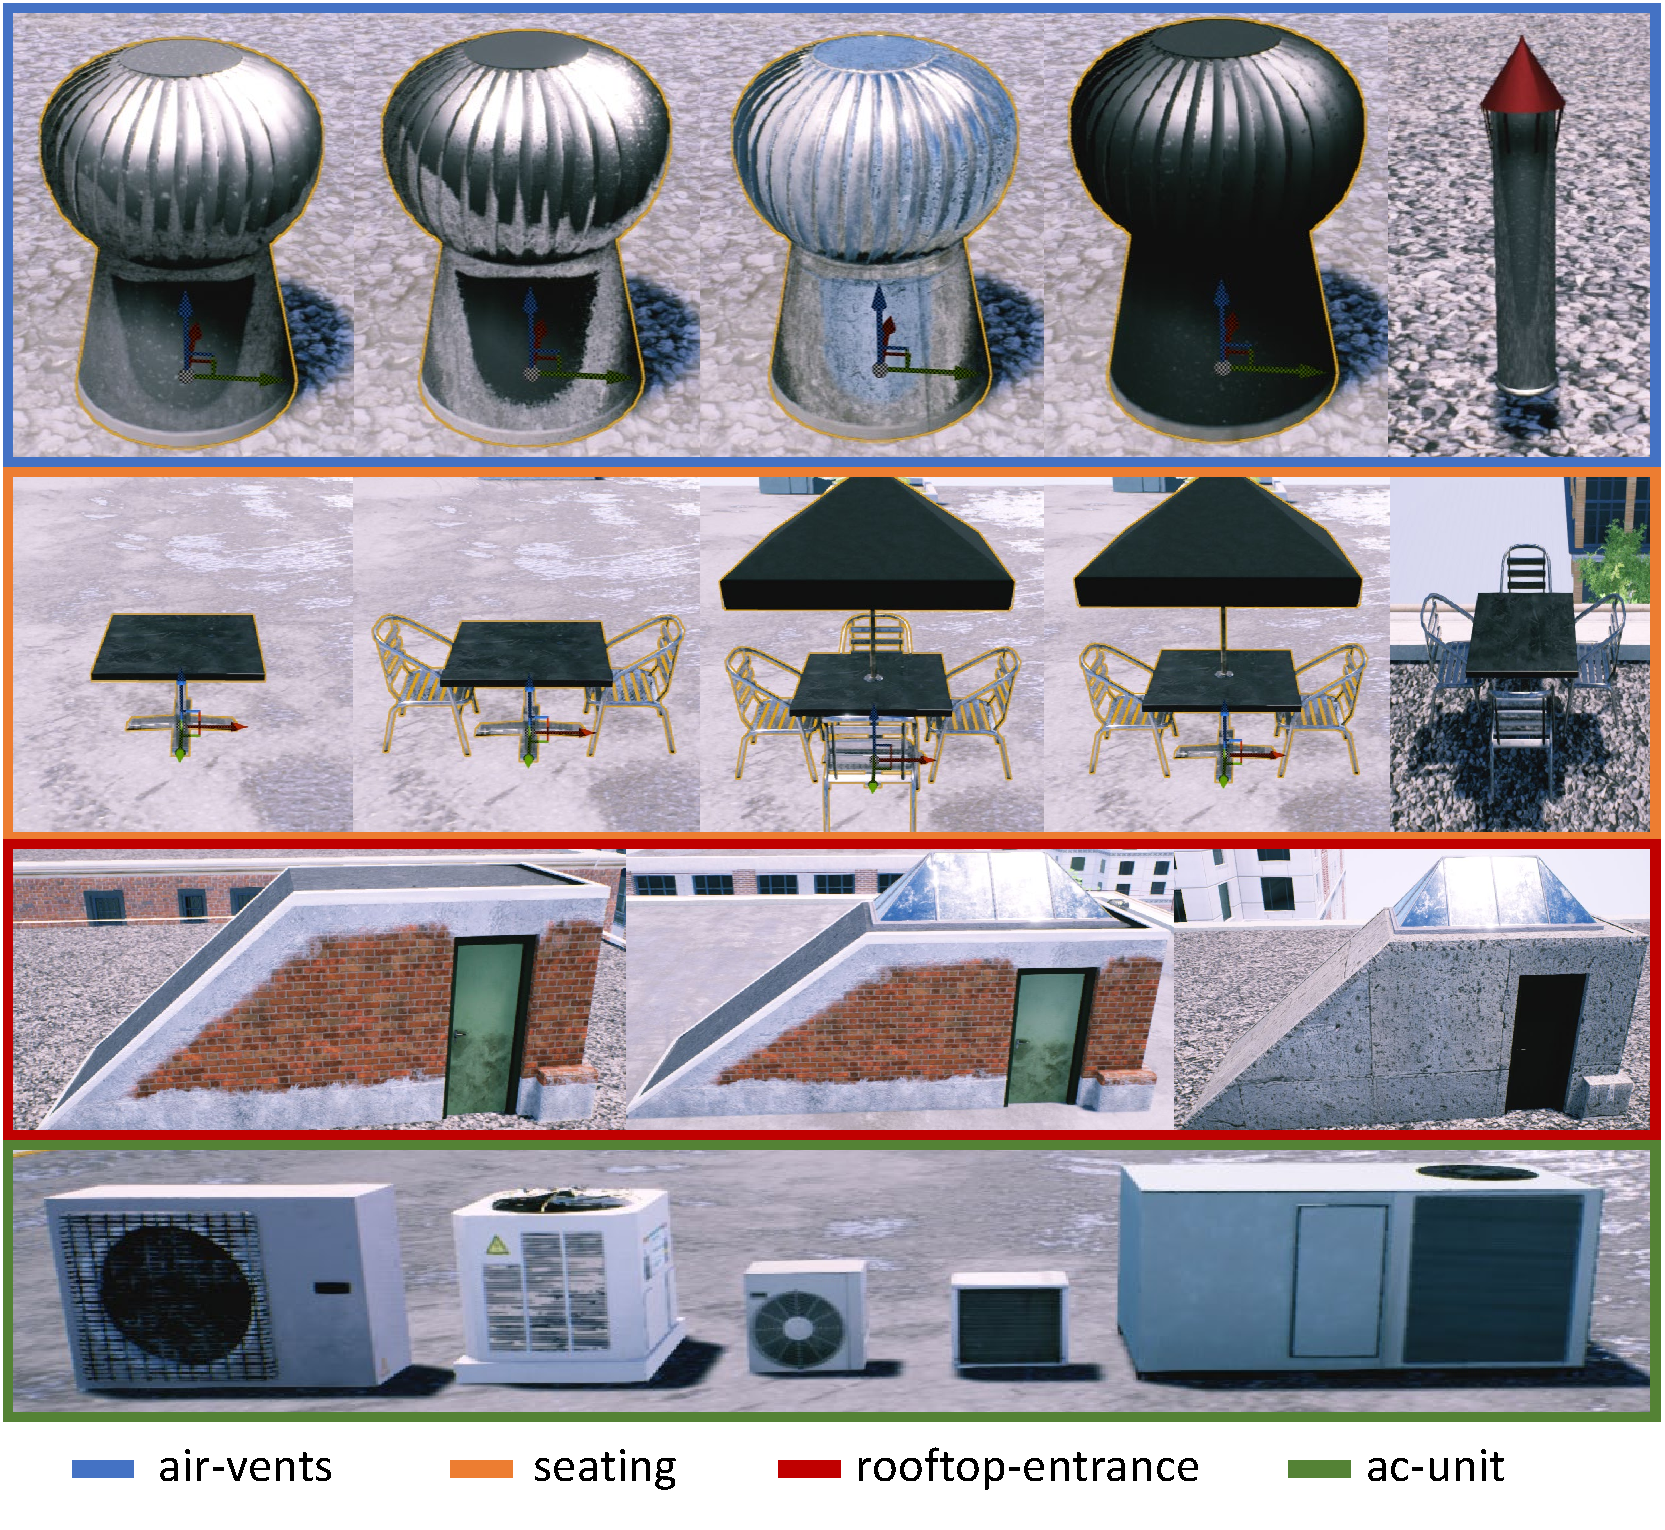
\includegraphics[width=.60\linewidth]{chapter_6_landingsim/figs/assets_all.pdf}
\caption[Examples of rooftop asset modelling and customization]{Examples of four rooftop assets (air-vents, seating, rooftop-entrance, ac-unit) and a subset of their customization in random worlds. Metallic, texture, and static mesh properties can be altered for each asset type.  }
% Two different sampling techniques are shown, directly sampling from a histogram (orange) and sampling from a fitted kernel density estimator (blue)
\label{fig:ch6_all_assets}
\end{figure}


\begin{figure}[ht]
 \centering
  \begin{subfigure}{.40\linewidth}
    \centering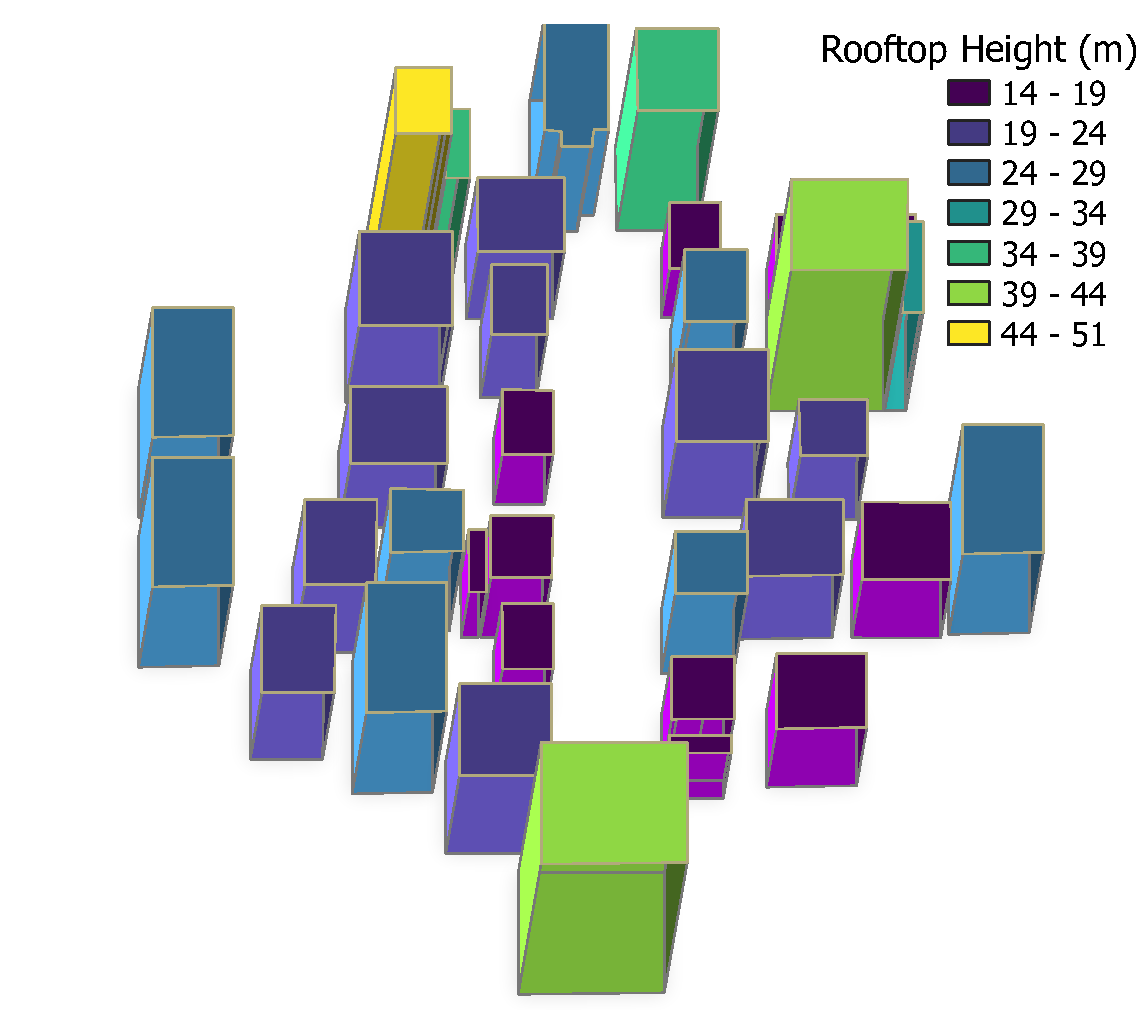
\includegraphics[page=1, width=.99\linewidth]{chapter_6_landingsim/figs/rooftop-map-3d.pdf}
    \caption{\label{fig:ch6_map_base_a}}
  \end{subfigure}
  \begin{subfigure}{.34\linewidth}
    \centering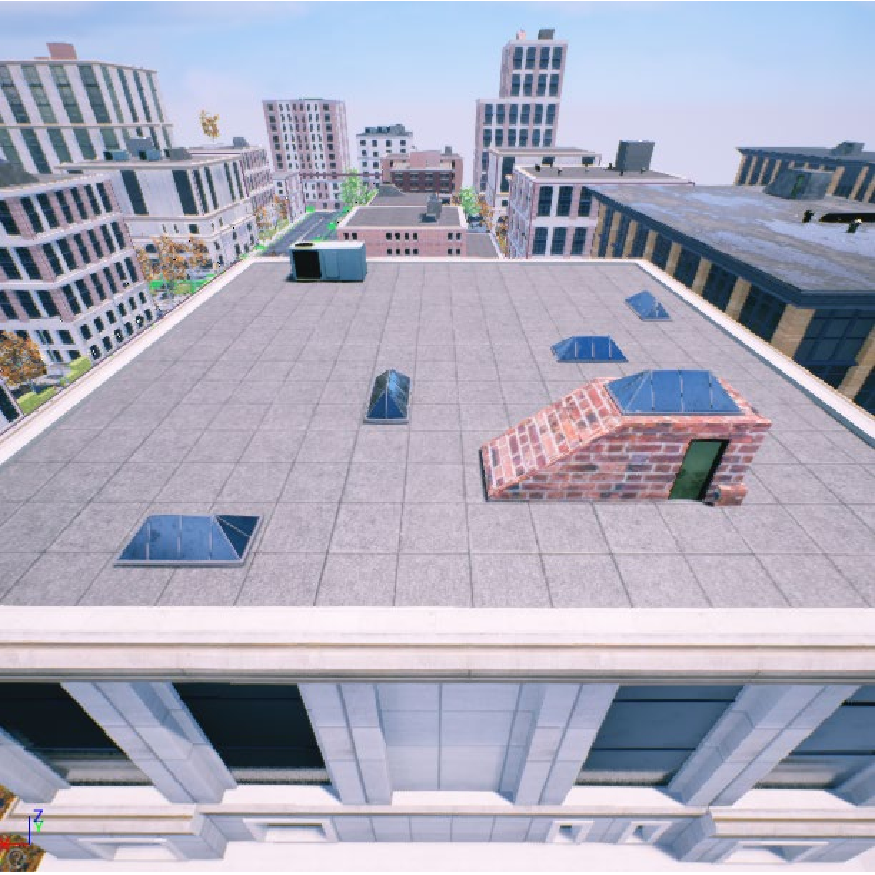
\includegraphics[page=1, width=.99\linewidth]{chapter_6_landingsim/figs/HistogramRoof.pdf}
    \caption{\label{fig:ch6_map_base_b}}
  \end{subfigure}
  \caption[Example simulated urban city]{ (\subref{fig:ch6_map_base_a}) Map of the 33 base city flat rooftops colorized by height. (\subref{fig:ch6_map_base_b}) Example of randomized asset placement from world generation script.}\label{fig:ch6_map_base}
\end{figure}

% was performed and leads to a more realistic world in terms of asset quantities, though placement could still be considered odd.
\subsection{Vehicle, Camera, and  LiDAR Models}

The vehicle model and simulator physics engine were provided by the AirSim plugin for Unreal Engine. The model treats an aircraft as a rigid body with $k$ actuators generating forces and torques. Details of the model and physics engine are found in Ref. \cite{shah_airsim_2018}. AirSim generates UAS-based camera and LiDAR sensor data feeds. The camera uses a pinhole camera model with configurable random noise. The LiDAR sensor is modeled as a spinning set of $n_l$ beams distributed equally within a vertical angular field of view (VFOV) and rotates clockwise within a horizontal field of view (HFOV). Simulated beam distance is calculated exactly and perfectly using ray casting. The authors found this model insufficient because it lacked noise and did not output an organized structure of point cloud data (i.e., range image) as spinning LiDAR systems provide. Therefore the LiDAR model was modified to resolve these two issues as described below.

Figure \ref{fig:ch6_lidar_errror} shows the LiDAR and error model developed in this work. Each beam is defined by spherical coordinates with a range ($d$), azimuth angle ($\theta$), and fixed elevation angle ($\phi$).  A properly-calibrated spinning LiDAR system has many forms of error including but not limited to range and encoder noise.  Drawing inspiration from Refs. \cite{schaefer_maximum_2019, koenig_design_2004}, our LiDAR model assumes the radial and azimuth error is distributed by zero-mean Gaussian noise, $e_d$ and $e_{\theta}$, respectively. Ref. \cite{glennie_static_2010} verifies this assumption holds for an angle of incidence below a critical angle, found to be $\sim 65^\circ$. This reference also showed a calibrated 64-beam Velodyne sensor had range and azimuth RMSE of approximately 3.2 cm and $0.03^{\circ}$, respectively.  We adopt similar values in our simulations.
\begin{figure}[ht!]
\centering

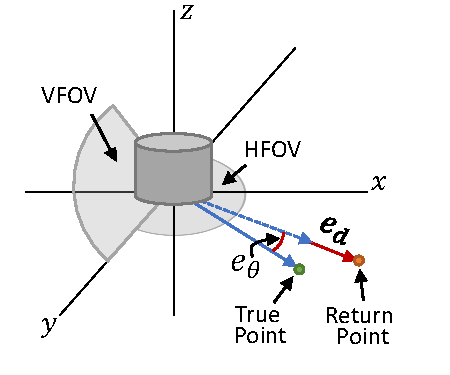
\includegraphics[clip,trim=0cm 0.5cm 0.5cm 0cm,, width=.40\linewidth]{chapter_6_landingsim/figs/LiDAR_Error.pdf}
\caption[LiDAR model used in simulation]{LiDAR model used in simulation. Error model account for range ($e_d$) and azimuth ($e_\theta$) error. }
% Two different sampling techniques are shown, directly sampling from a histogram (orange) and sampling from a fitted kernel density estimator (blue)
\label{fig:ch6_lidar_errror}
\end{figure}

The simulated LiDAR used in our work is configured with $n_l=64$ beams with a VFOV = $(-45^{\circ}, 45^{\circ})$ and a HFOV=$(-45^{\circ}, 45^{\circ})$. A scan is collected after the full HFOV is traversed and recorded as an organized point cloud, with $n_l$ rows and $n_c$ columns, where  $n_c$ is fixed and determined by the scanning and rotation rate:
$$
n_c = \frac{90^{\circ}}{360^{\circ}} \cdot \frac{\text{PointsPerSecond}}{\text{RotationsPerSecond} } \cdot \frac{1 \text{Beam}}{64 \text{Beam}}
$$

Rotation rate was set to 20Hz with 655360 points per seconds as modeled from an Ouster OS0 sensor\cite{ouster_os0}. Note that this LiDAR model, like Refs. \cite{schaefer_maximum_2019, koenig_design_2004}, does not account for LiDAR motion distortion for a moving vehicle. However, motion distortion can be removed through efficient processing using feature scanning with an on-board inertial measurement unit (IMU) \cite{mohamed_survey_2019, zhang_point_2019}. Additionally, this work assumes the drone is in a stable hover such that it can ignored in this model.

\section{Semantic Segmentation Results}\label{sec:ch6_segmention_results}

\subsection{Creating image dataset}

Training, validating, and testing a neural network to segment rooftops and obstructions requires a large annotated image dataset. To accomplish this we first generated eight random worlds used for training the neural network.  The world generation script was seeded with different numbers generating different random worlds. Each world assumed equal likelihood for all asset placement leading to rich and diverse rooftop assets. Note that the buildings and lighting conditions are held constant, only rooftop assets are different in each world. An image collection script was created that captured images of rooftops and their obstructions with corresponding ground truth segmentation labels.  The images are captured at a variety of positions and orientations pointed at the center of the rooftops as shown in Figure \ref{fig:ch6_sampling_strategy}. The blue arrows represent the position and direction of the camera while the green rectangle denotes the rooftop. A sphere centered at the rooftop with a radius five meters greater than the rooftops radial footprint fixes these sampling configurations. A total of 11,989 images were collected and split 80/20 into a training and validation set, respectively. The test set was created in a similar manner except from random worlds following the asset quantity distribution recorded from the Manhattan dataset.  A weighted sampling procedure was used where the weights were directly used from the data histogram per \cite{Efraimidis2008}. A total of 5,465 images were collected for the test dataset.

\begin{figure}[ht!]
\centering
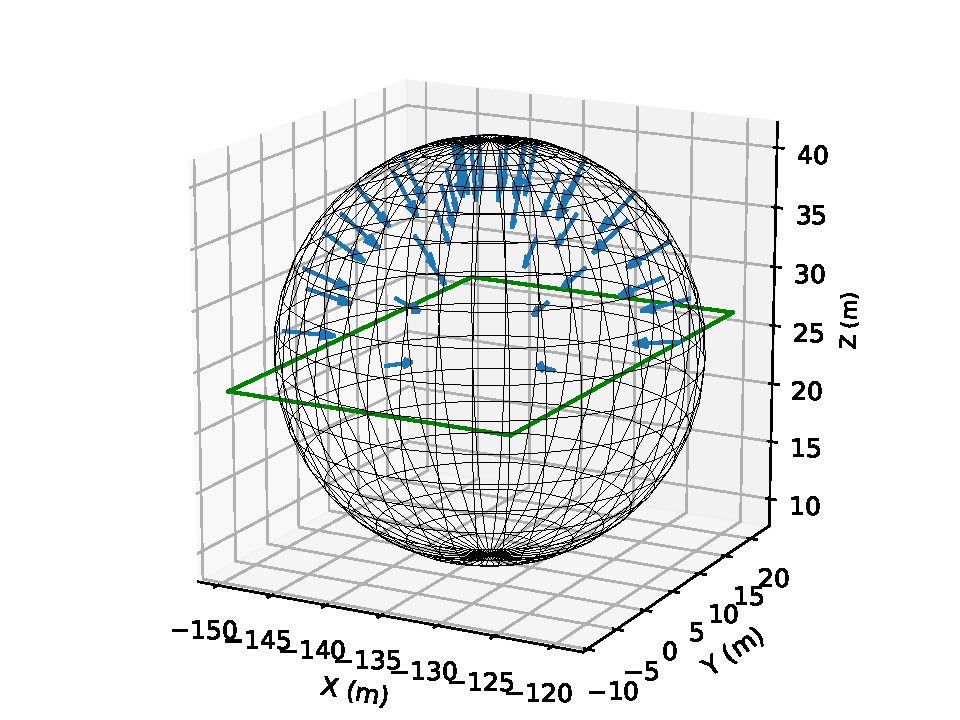
\includegraphics[clip,trim=1cm 0.0cm 0.0cm 1cm,, width=.50\linewidth]{chapter_6_landingsim/figs/SamplingSphere.pdf}
\caption[Image sampling strategy for rooftops]{Image sampling strategy for creating an annotated dataset of rooftop segmentation. Blue arrows denote the position and orientation of the camera. The green polygon denotes the rooftop.}
% Two different sampling techniques are shown, directly sampling from a histogram (orange) and sampling from a fitted kernel density estimator (blue)
\label{fig:ch6_sampling_strategy}
\end{figure}

\subsection{Training and Testing Results}

\xhdr{Implementation details:} We evaluated four combinations of CNN backbones and decoders for
image semantic segmentation: MobileNet + FCN8s, ShuffleNet + FCN8s, MobileNet + UNet, and ShuffleNet + UNet. We
modified models based on tensorflow implementations~\cite{siam_comparative_2018} and perform training and testing on a system with an Nvidia RTX 2080
GPU. Each model was trained for 100 epochs with early stopping enabled using the validation dataset.

\xhdr{Metrics:} We evaluate mean intersection over union (IoU)
and per-class IoU for each method on the test dataset.

\xhdr{Quantitative results:} As can be seen in Table~\ref{tab:segmentation_results}, the
MobileNet + UNet model achieves the best mean IoU and the
best per-class IoU on most cases while MobileNet+FCNs
performs the second best in most Table II cases. Specifically
both models outperform the ShuffleNet based methods on
small-rooftop-entrance, skylight, air-vents and ac-units which
appear frequently in the real world and are more important
to rooftop landing tasks. The trained MobileNet + UNet model is chosen for performing semantic segmentation to evaluate our proposed methods.
\begin{table*}[htbp]
    \centering
    \caption[Semantic segmentation accuracy results]{The per-class IoU and mean IoU of different image semantic segmentation networks on our urban rooftop dataset. The top mean IoU is highlighted in bold. The chimney class is absent from the test dataset so its IoUs are not available.}
    \resizebox{1.0 \textwidth}{!} {
    \begin{tabular}{c|ccccccccccccc|c}
        \toprule
         & sky & ground & \makecell{building \\wall} &  \makecell{building \\rooftop} &  \makecell{small \\rooftop \\entrance} &  \makecell{sky\\light} &  \makecell{air-\\vents} &  \makecell{ac-\\unit} & seating &  \makecell{air-\\ducts} &  \makecell{water\\tower} & tarp & vegetation & \makecell{Mean\\ IoU}\\
         \midrule
         \makecell{MobileNet\\+ FCN8s} & 0.99 & 0.93 & 0.96 & 0.98 & 0.82 & 0.79 & 0.48 & 0.78 & 0.42 & 0.80 & 0.74 & 0.90 & 0.81 & 0.74 \\
         \makecell{ShuffleNet \\+ FCN8s} & 0.99 & 0.92 & 0.95 & 0.97 & 0.78 & 0.76 & 0.41 & 0.75 & 0.37 & 0.73 & 0.68 & 0.84 & 0.79 & 0.71\\
         \makecell{MobileNet \\+ UNet} & 0.99 & 0.93 & 0.97 & 0.98 & 0.83 & 0.84 & 0.50 & 0.81 & 0.47 & 0.81 & 0.78 & 0.84 & 0.90 & \textbf{0.76}\\
         \makecell{ShuffleNet \\+ UNet} & 0.99 & 0.94 & 0.96 & 0.98 & 0.79 & 0.79 & 0.36 & 0.77 & 0.34 & 0.74 & 0.76 & 0.91 & 0.88 & 0.73\\
        \bottomrule
    \end{tabular}
    }
    \label{tab:segmentation_results}
\end{table*}

\section{Touchdown Point Selection Results} \label{sec:ch6_touchdown_point_results}

Our proposed touchdown point selection procedure was evaluated in a newly generated simulated city environment not used for training the semantic segmentation neural network. The rooftop assets are newly randomized and follow the asset quantity distribution of Manhattan. The full parameters used for Semantic Polylidar3D are shown in Table \ref{table:polylidar3D_params}. Please see \cite{castagno_polylidar3d_2020} for a full explanation of selected parameters. Note that $\theta_{max}$ and $vert_{min}$ are new parameters governing semantic integration in polygon extraction as described in Section \ref{sec:ch6_methods_semantic_polylidar3d}. The LiDAR model was configured with 64 beams/channels with range and azimuth error of 5 cm and 0.1 degrees, respectively. The camera image size was 500 $\times$ 500. 
% The error tolerance for finding the greatest inscribed circle in a returned polygon was set to 10 cm.   

\begin{table}[ht]
\centering
\caption{Semantic Polylidar3D Parameters}\label{table:polylidar3D_params}
\begin{tabular}{@{}ll@{}}
\toprule
Algorithm        & Parameters                                                          \\ \midrule
Laplacian Filter & $\lambda$=0.65, kernel=3, iterations=1   \\
Bilateral Filter & $\sigma_l$=0.3, $\sigma_a$=0.2, kernel=3, iterations=4 \\
FastGA           & level=5,  $v_{min}$=50, $d_{peak}$=0.28            \\
                 & $sample_{pct}$=50\% \\
Plane/Poly Extr. & $tri_{min}$=500,  $l_{max}$=1.5, $\theta_{min}$=0.96 \\
                 & $ptp_{max} = 0.2$, $vertices^{hole}_{min}$ = 4  \\
                 & $\mathbf{\theta_{max} = 0.90, vert_{min}= 2}$ \\
Poly. Filtering  & $\alpha = 0.25$ , $\beta_{pos}$ = 0.1, $\beta_{neg}$ = 0.25, \\
                 & $\gamma$ = 4, $\delta$ = 0.1      \\ \bottomrule
\end{tabular}
\end{table}

Two analyses were performed that quantified the accuracy and speed of Semantic Polylidar3D and evaluated the maximum height before obstacle identification failures occurred (decision height).  Each is described below.

\subsection{Semantic Polylidar3D Accuracy and Speed} \label{sec:ch6_landing_accuracy}

\subsubsection{Creating Test Data}

LiDAR and camera image data were collected at 10 meters above each of the 33 rooftops. For each rooftop, the drone was positioned and orientated in five different configurations.  One configuration is at the center of the rooftop with the drone aligned with the $x$-axis. The other four configurations are offset from the rooftop center $\pm5$ meters in both the $x/y$ axes with the drone facing towards the rooftop center. The drone is assumed in a stable level hover with sensors pointing down as described above. Each configuration gathers two samples, providing a total of $330$ independent samples. A sample consists of a LiDAR scan and an image from the monocular camera. The LiDAR has random noise making the two samples independent. To assess accuracy, ground truth polygons including obstacles were required for each rooftop. However, the field of view of the LiDAR and camera sensors are limited thus may not contain the full rooftop. Fig. \ref{fig:ch6_clipping_a} shows the ground truth polygon of the rooftop (green/orange), the classified point cloud, and the FOV of the camera sensor (red frustum). To resolve this issue the ground truth polygon is clipped to the camera field of view as shown in Fig. \ref{fig:ch6_clipping_b}. This same clipping procedure is also performed on the output of predicted polygons. This allows any method to be fairly assessed from data within the the camera FOV. Accuracy is assessed as the Intersection over Union (IoU) of the predicted polygon and the clipped ground truth polygon. 

\begin{figure}[ht]
 \centering
  \begin{subfigure}{.40\linewidth}
    \centering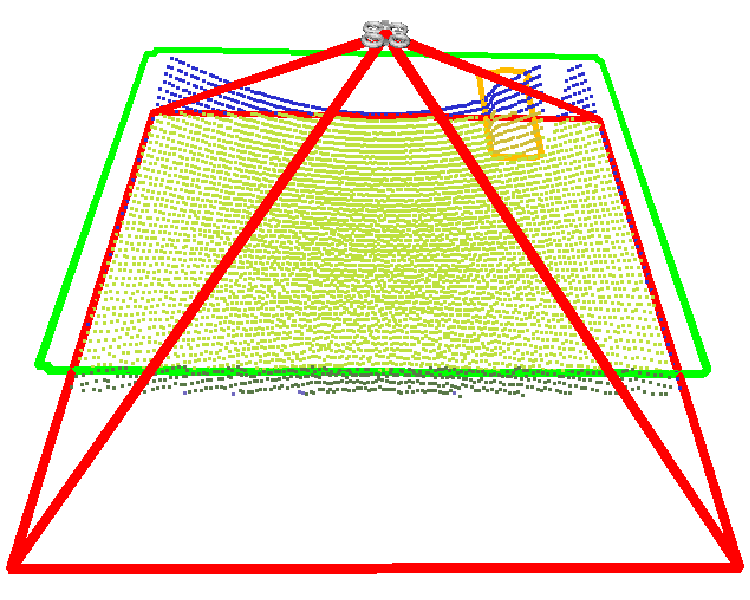
\includegraphics[page=1, width=.99\linewidth]{chapter_6_landingsim/figs/GroundTruthClipping.pdf}
    \caption{\label{fig:ch6_clipping_a}}
  \end{subfigure}
  \begin{subfigure}{.40\linewidth}
    \centering\includegraphics[page=2, width=.99\linewidth]{chapter_6_landingsim/figs/GroundTruthClipping.pdf}
    \caption{\label{fig:ch6_clipping_b}}
  \end{subfigure}
  \caption[Semantic Polylidar3D parameters]{ (\subref{fig:ch6_clipping_a}) Rooftop ground truth polygon (exterior=green,holes=orange), classified point cloud, and camera FOV frustum (red). (\subref{fig:ch6_clipping_b}) The ground truth polygon is clipped (purple) to be inside the frustum.}\label{fig:ch6_clipping}
\end{figure}



\subsubsection{Qualitative Results}

\begin{figure*}[!t]
 \centering
  \begin{subfigure}{.32\linewidth}
    \centering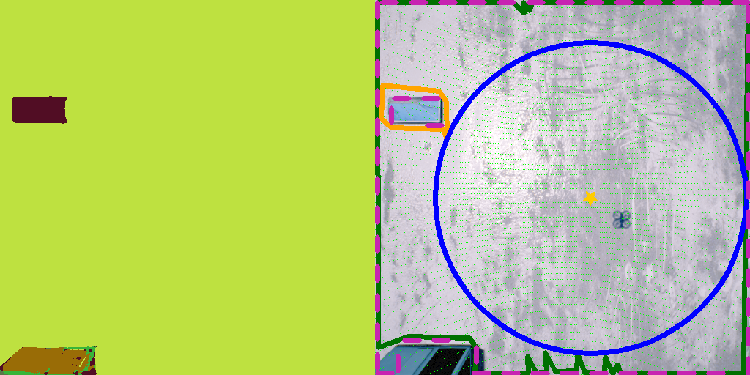
\includegraphics[page=1, width=.99\linewidth]{chapter_6_landingsim/figs/QualitativeExamples.pdf}
    \caption{\label{fig:ch6_qualitative_a}}
  \end{subfigure}
%   \begin{subfigure}{.45\linewidth}
%     \centering\includegraphics[page=2, width=.99\linewidth]{chapter_6_landingsim/figs/QualitativeExamples.pdf}
%     \caption{\label{fig:ch6_qualitative_b}}
%   \end{subfigure}
  \begin{subfigure}{.32\linewidth}
    \centering\includegraphics[page=3, width=.99\linewidth]{chapter_6_landingsim/figs/QualitativeExamples.pdf}
    \caption{\label{fig:ch6_qualitative_c}}
  \end{subfigure}
  \begin{subfigure}{.32\linewidth}
    \centering\includegraphics[page=4, width=.99\linewidth]{chapter_6_landingsim/figs/QualitativeExamples.pdf}
    \caption{\label{fig:ch6_qualitative_d}}
  \end{subfigure}
  \caption[Example touchdown point selection on rooftops]{Three examples of touchdown point selection. Predicted segmentation and camera image with overlaying projected polygons are shown on the left and right, respectively. Dashed purple lines represent ground truth polygons while green/orange represent the predicted polygon. The center of the blue circle is the selected touchdown point.     }\label{fig:ch6_qualitative}
\end{figure*}

Figure \ref{fig:ch6_qualitative} displays three examples of our touchdown point selection process, each with two images. The left image shows the neural network semantic classification map while the right image displays the camera image overlaid with polygons.  Semantic Polylidar3D polygons are shown in green/orange (orange is interior obstacles); the clipped ground truth polygons are indicated by a dashed purple line, and the center of the blue circle represents the optimal touchdown point. A safe touchdown point is found in each of these examples.  Generated polygons map reasonably to ground truth polygons but may overestimate the size of large obstacles such as the rooftop entrances seen in (c). This occurs when obstacles occlude perception by the camera and LiDAR sensors, leaving a ``shadow'' of missing information behind them. Our method is conservative in that such regions will not be considered touchdown options. 
% A full analysis on accuracy is provided in Sec. \ref{sec:ch6_landing_accuracy}.

Fig. \ref{fig:ch6_case1} demonstrates a challenging scenario where Semantic Polylidar3D does an excellent job of correctly identifying a landing site and selecting a touchdown point. This building has a rooftop-entrance as well as a slightly non-planar (wrinkled) tarp on its surface as shown in (a). The rooftop-entrance has a concrete-like texture that is similar to the texture of the rooftop itself. At a distance (e.g., 10 m) they look nearly identical which causes a neural network segmentation failure as shown in (b). However, because both LiDAR and vision are used in the Semantic Polylidar3D algorithm,  failure in one modality did not lead to a failure in identifying the rooftop entrance. The orange obstacle line fully encapsulates the rooftop-entrance as shown in (c). In addition, the neural network was able to correctly identify the tarp allowing Semantic Polylidar3D to exclude the tarp from the landing site polygon. The tarp is outside the polygon boundary in (c). Baseline Polylidar3D shown in (d) only uses LiDAR and is not able to fully identify the tarp obstacle because its planarity is similar to the ground. Only a small section on the border is captured as an interior hole. This example shows Semantic Polylidar3D's increased robustness to neural network errors in vision and range error from LiDAR by fusing modalities during polygon extraction. 

\begin{figure}[ht]
 \centering
  \begin{subfigure}{.25\columnwidth}
    \centering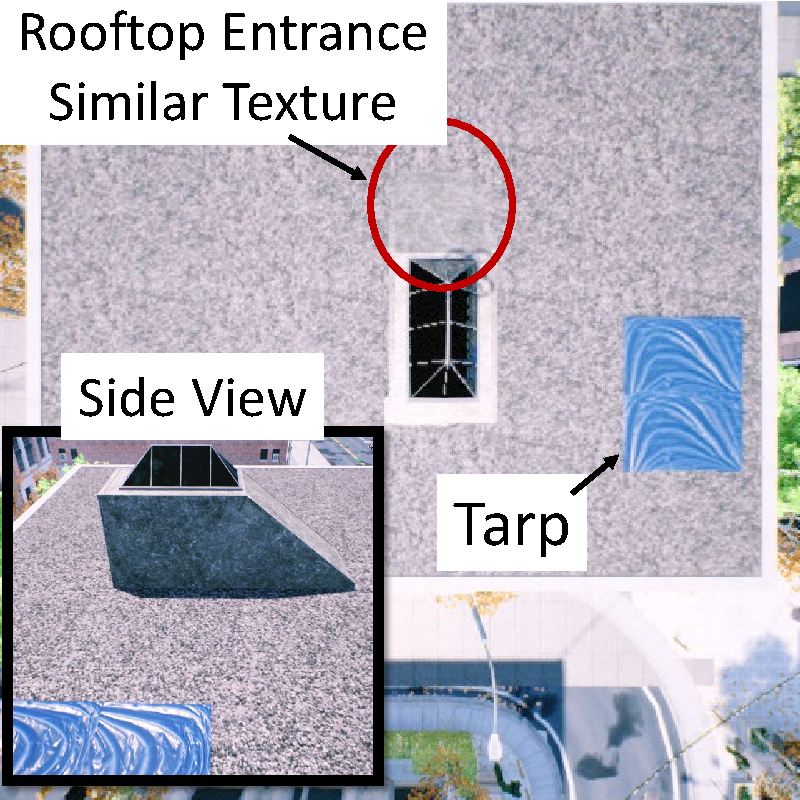
\includegraphics[page=1, width=.99\columnwidth]{chapter_6_landingsim/figs/CompareAlgs_Case1.pdf}
    \caption{\label{fig:ch6_case1_a}}
  \end{subfigure}
%   \begin{subfigure}{.32\linewidth}
%     \centering\includegraphics[page=2, width=.99\linewidth]{chapter_6_landingsim/figs/CompareAlgs_Case1.pdf}
%     \caption{\label{fig:ch6_case1_b}}
%   \end{subfigure}
  \begin{subfigure}{.25\columnwidth}
    \centering\includegraphics[page=3, width=.99\columnwidth]{chapter_6_landingsim/figs/CompareAlgs_Case1.pdf}
    \caption{\label{fig:ch6_case1_c}}
  \end{subfigure}
 
  \begin{subfigure}{.25\columnwidth}
    \centering\includegraphics[page=5, width=.99\columnwidth]{chapter_6_landingsim/figs/CompareAlgs_Case1.pdf}
    \caption{\label{fig:ch6_case1_d}}
  \end{subfigure}
  \begin{subfigure}{.25\columnwidth}
    \centering\includegraphics[page=4, width=.99\columnwidth]{chapter_6_landingsim/figs/CompareAlgs_Case1.pdf}
    \caption{\label{fig:ch6_case1_e}}
  \end{subfigure}
  \caption[Example of Semantic Polylidar3D on a challenging rooftop]{ (\subref{fig:ch6_case1_a}) Rooftop with tarp and rooftop-entrance. The entrance texture is similar to the rooftops.  (\subref{fig:ch6_case1_c}) Neural network semantic segmentation. 
   (\subref{fig:ch6_case1_d}) Proposed Semantic Polylidar3D polygon extraction. (\subref{fig:ch6_case1_e}) Baseline Polylidar3D fails to identify the tarp. }\label{fig:ch6_case1}
\end{figure}


\subsubsection{Accuracy Assessment}

The IoU of the predicted polygon and ground truth polygon (clipped to camera FOV) is computed for each sample to assess accuracy. We also compare these results with baseline Polylidar3D which only uses LiDAR data in flat surface extraction. Figure \ref{fig:ch6_compare_algs} shows overlaying histograms and kernel density estimators of the IoU results where blue and orange denote the baseline against our new proposed method, respectively. Above the histogram are the respective mean and $\sigma$ error bars. Semantic Polylidar3D has a mean and sigma of $91.2 \pm 4\%$ against baseline Polylidar3D with $86.8 \pm 6\%$. A T-test was conducted between each group giving a t-statistic of 11.0 with a p-value $<$ 0.001. These results indicate a substantial improvement in touchdown point selection with Semantic Polylidar3D's integration of computer vision and computational geometry methods. 

% indicating the differences between these methods is 11X greater than the differences within them.

\begin{figure}[ht!]
\centering
% 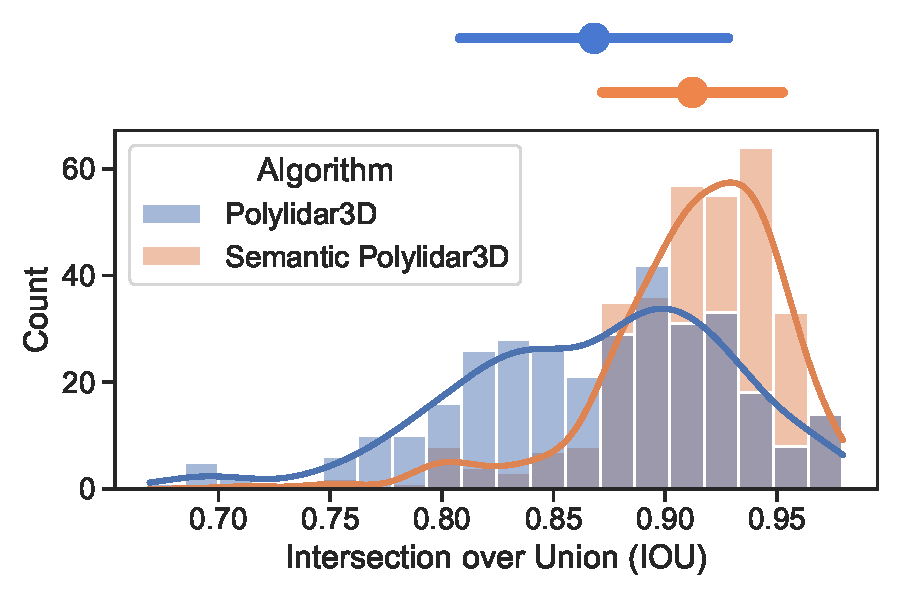
\includegraphics[width=.85\linewidth]{chapter_6_landingsim/figs/compare_algs_extra_2.pdf}
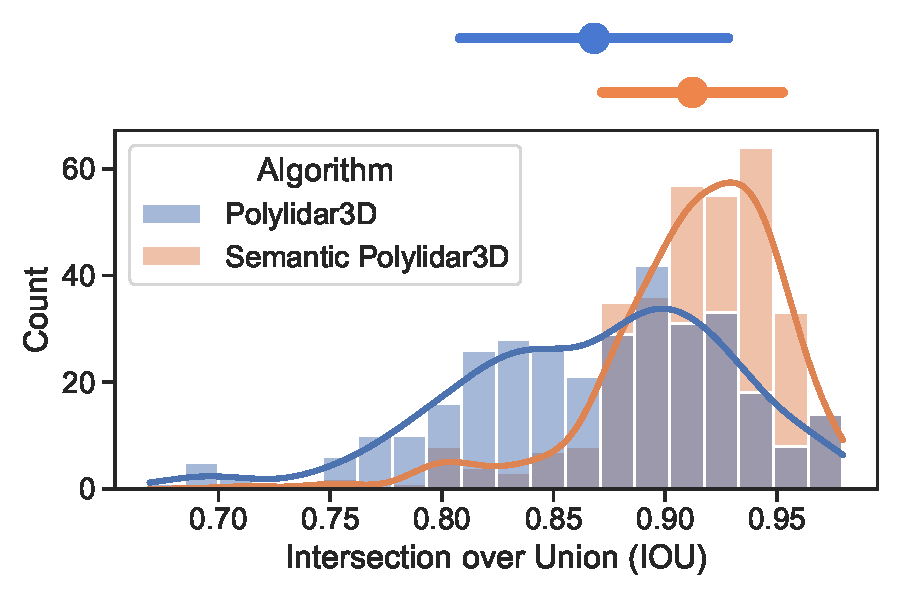
\includegraphics[width=.55\linewidth]{chapter_6_landingsim/figs/compare_algs_extra_2.pdf}
\caption[Accuracy benchmark for Semantic Polylidar3D]{Accuracy of Polylidar3D (blue, baseline) versus Semantic Polylidar3D (orange, proposed). A higher IoU indicates the algorithm captured more of the surface and correctly identified obstacles. Mean and $1\sigma$ bars are shown on top.}
% Two different sampling techniques are shown, directly sampling from a histogram (orange) and sampling from a fitted kernel density estimator (blue)
\label{fig:ch6_compare_algs}
\end{figure}

\subsubsection{Execution Time}

Table \ref{table:execution Time} displays the mean and $1\sigma$ execution time in milliseconds for all major steps in the proposed touchdown point selection algorithm. The GPU accelerated neural network segmentation is the most time consuming portion. Note that no optimization techniques have been performed such as quantizing the segmentation model or reducing the number of classes. The total execution time of the method is sufficiently low to be executed in near real-time with UAS sensor data streams. 


\begin{table}[ht]
\centering
\caption{Execution Time (ms)} \label{table:execution Time}
\begin{tabular}{@{}p{1.9cm}p{1.9cm}p{1.9cm}p{1.9cm}cc@{}}
\toprule
Segment Image  & Classify Points & Semantic Polylidar  & Touchdown Site & Total\\ \midrule
$21.2 \pm 1.1$& $1.7 \pm 0.1$   & $9.5 \pm 1.5$   & $0.1$ & $32.6 \pm 1.8$      \\ \bottomrule
\end{tabular}

\end{table}

% \subsection{Contingency Planning}

\subsection{Decision Height Analysis}

Landing decision height for VTOL aircraft refers to the height needed to limit glide slope and trajectory tracking errors to smoothly transition from approach to a stable hover over a touchdown point \cite{hoh_decision-height_1991}.  This height depends on vehicle performance characteristics, local environmental conditions (e.g. wind speed), and sensor errors. The touchdown point selection algorithm proposed in this manuscript must handle some error from both visual and range sensors as well as neural network segmentation.  We performed a series of experiments that determined the maximum hover height at which our proposed algorithm can accurately identify a human on a rooftop as an obstacle as shown in Figure \ref{fig:ch6_dp_a}.

The same simulation and algorithm parameters described in Section \ref{sec:ch6_landing_accuracy} were used for this evaluation. A multi-factor experiment was conducted over hover height set (5, 10, 15, 20, 25, 30) meters and LiDAR sensor set (16, 32, 64) beams, respectively. The drone hovered at each height level and covered a constant-height $2\times2$ meter grid directly above the person. The drone observed the rooftop from 25 positions within the grid, positioning itself at 0.5 meter intervals. At each observation point the roof and obstacle were extracted using Semantic Polylidar3D. The highest height level where $\frac{24}{25}$ observation points correctly captured the human as an obstacle are shown in Table \ref{table:decision_height}. The greater the number of beams, the higher the point cloud coverage of the human rooftop ``obstacle''. Note that at $\approx 25$ meters the person appears as only a few pixels in a $500\times500$ camera image such that the neural network is unable to distinguish the person from the roof. This means a camera can not solely detect the person at or above 25 meters.

\begin{table}[!ht]
\centering
\caption{Maximum height for LiDAR to identify a human on the roof.} \label{table:decision_height}
\begin{tabular}{@{}cccc@{}}
\toprule
                & 16 Beams & 32 Beams & 64 Beams \\ \midrule
Decision height & 10 m     & 20 m     & 30 m     \\ \bottomrule
\end{tabular}
\end{table}

\begin{figure}[ht]
 \centering
%   \begin{subfigure}{.45\linewidth}
  \begin{subfigure}{.35\linewidth}
    \centering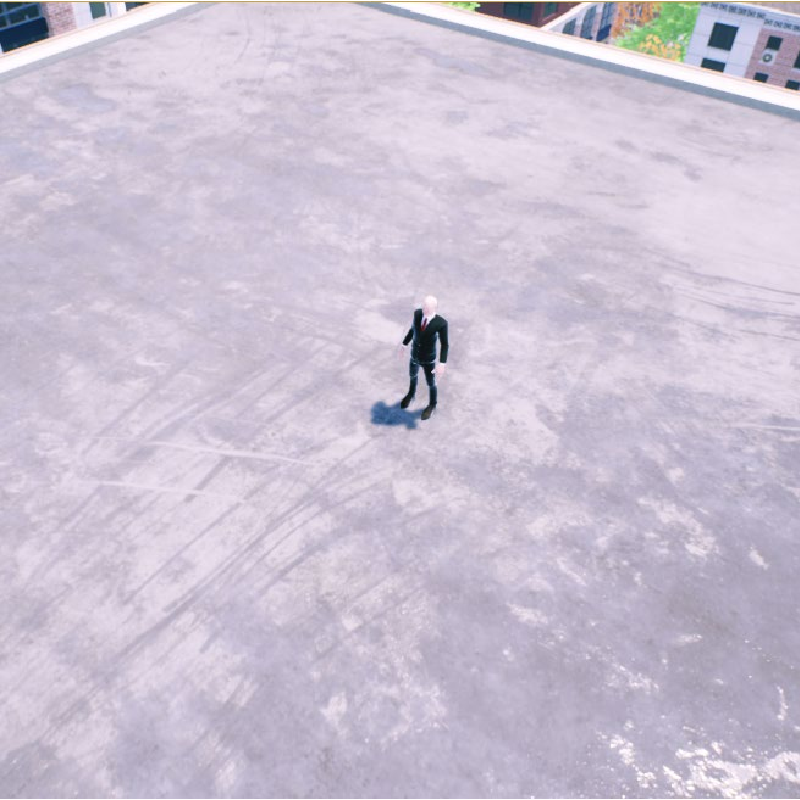
\includegraphics[page=1, width=.99\linewidth]{chapter_6_landingsim/figs/DecisionPointImages.pdf}
    \caption{\label{fig:ch6_dp_a}}
  \end{subfigure}
%   \begin{subfigure}{.45\linewidth}
  \begin{subfigure}{.35\linewidth}
    \centering\includegraphics[page=2, width=.99\linewidth]{chapter_6_landingsim/figs/DecisionPointImages.pdf}
    \caption{\label{fig:ch6_dp_b}}
  \end{subfigure}
  \caption[Rooftop environment for decision height analysis]{ (\subref{fig:ch6_dp_a}) Rooftop environment for decision height analysis.   (\subref{fig:ch6_dp_b}) Example observation point of a drone five meters above a person.}\label{fig:ch6_dp}
\end{figure}

\section{Discussion}\label{sec:ch6_discussion}

The presented results demonstrate that Semantic Polylidar3D offers improvement in accurately identifying touchdown points over a purely geometric method. Overall Semantic Polylidar3D had a 4\% improvement in IoU accuracy compared to the geometric baseline. Additionally, Figure \ref{fig:ch6_compare_algs} shows that adding semantic information has reduced the long tail distribution of low accuracy/worst case examples. The results show our proposed method is robust to individual sensor failures as seen in Figure \ref{fig:ch6_case1}. For example, a segmentation failure to identify an obstacle does not lead to total failure unless it is also missed by the LiDAR sensor. Additionally, successful identification of a rooftop using the neural network attenuates range noise by reducing geometric constraints to reduce false negatives.

The total execution of the touchdown point selection pipeline takes $\approx$ 30 ms, strictly dominated by the neural network. It is likely this execution time can be significantly reduced with model quantization, simplification, and limiting/retraining the network to binary segmentation to identify rooftop / non-rooftop surfaces only.

The archived map for safe rooftop landing sites must be updated when the sensor-based planner fails to find a safe touchdown point during the 10m hovering rooftop scans described in this work.  The ``live polygons'' (LP) extracted from the onboard sensor can be used to resolve the inaccuracies in the ``archival polygon'' (AP) of the rooftop. First, the LP of the landing surface (if it exists) must be transformed from the sensor frame to GPS coordinates to align with the map data. This requires the aircraft to have onboard GPS with sufficient localization accuracy.  Figure \ref{fig:ch6_map_upate} shows an example of an archival and live polygon in (a) and (b), respectively. The archival and live polygon are intersected to create an intersection polygon (IP) shown in (c). This gives the most conservative estimate for observable landing area that can be updated. The camera FOV is overlaid in red. Finally an updated polygon (UP) is created through the union of the IP with the AP subtracted from the FOV. Camera FOV limits the scope of area available for updating. 

% The sequence of operations are:
% \begin{equation*}
%     IP =  LP \cap AP \\
%     \ \ \ UP = IP \cup (AP - FOV)
% \end{equation*}

\begin{figure}[ht]
 \centering
  \begin{subfigure}[t]{.30\linewidth}
    \centering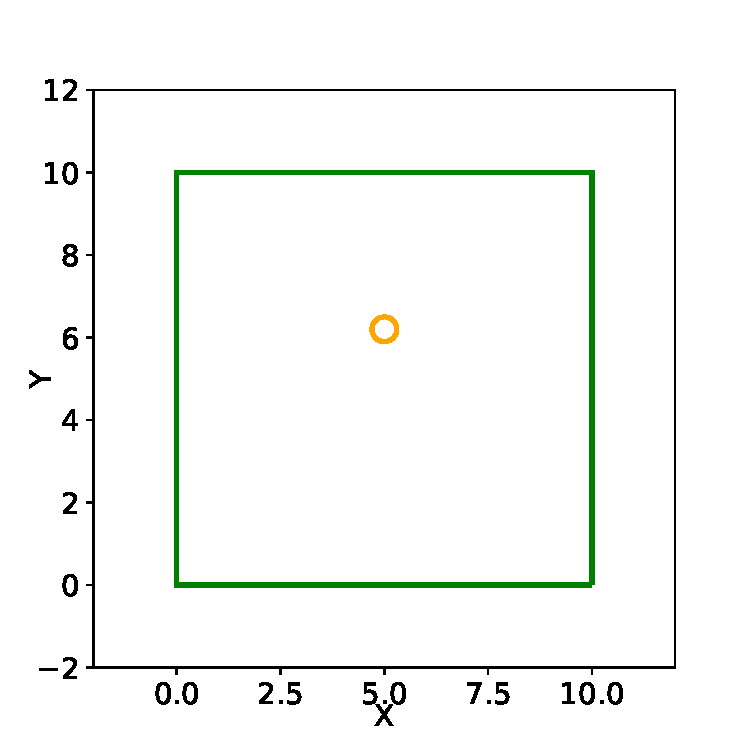
\includegraphics[clip, trim=0cm 0cm 0.0cm 0cm, width=.99\linewidth]{chapter_6_landingsim/figs/map_update_a.pdf}
    \caption{Archival Polygon (AP)\label{fig:ch6_map_update_a}}
  \end{subfigure}
  \begin{subfigure}[t]{.30\linewidth}
    \centering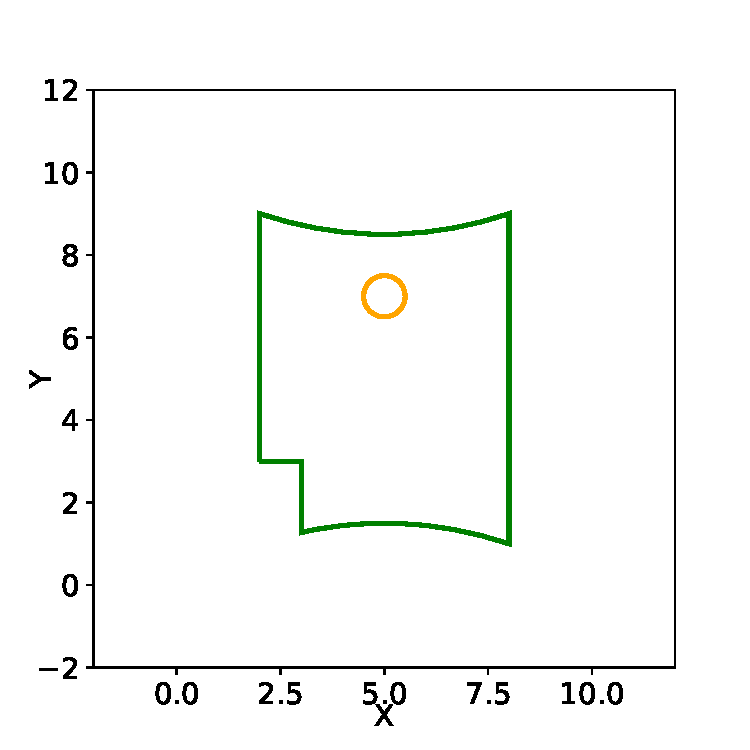
\includegraphics[clip, trim=0cm 0cm 0.0cm 0cm, width=.99\linewidth]{chapter_6_landingsim/figs/map_update_b.pdf}
    \caption{Live Polygon (LP)\label{fig:ch6_map_update_b}}
  \end{subfigure}
  
  \begin{subfigure}[t]{.30\linewidth}
    \centering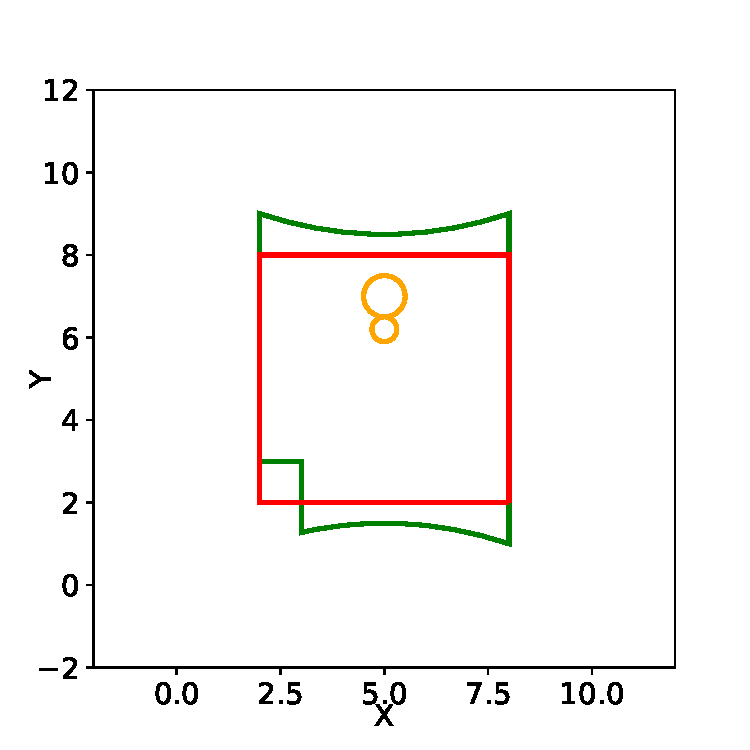
\includegraphics[clip, trim=0cm 0cm 0.0cm 0cm, width=.99\linewidth]{chapter_6_landingsim/figs/map_update_c.pdf}
    \caption{Intersection Polygon (IP)\label{fig:ch6_map_update_c}}
  \end{subfigure}
  \begin{subfigure}[t]{.30\linewidth}
    \centering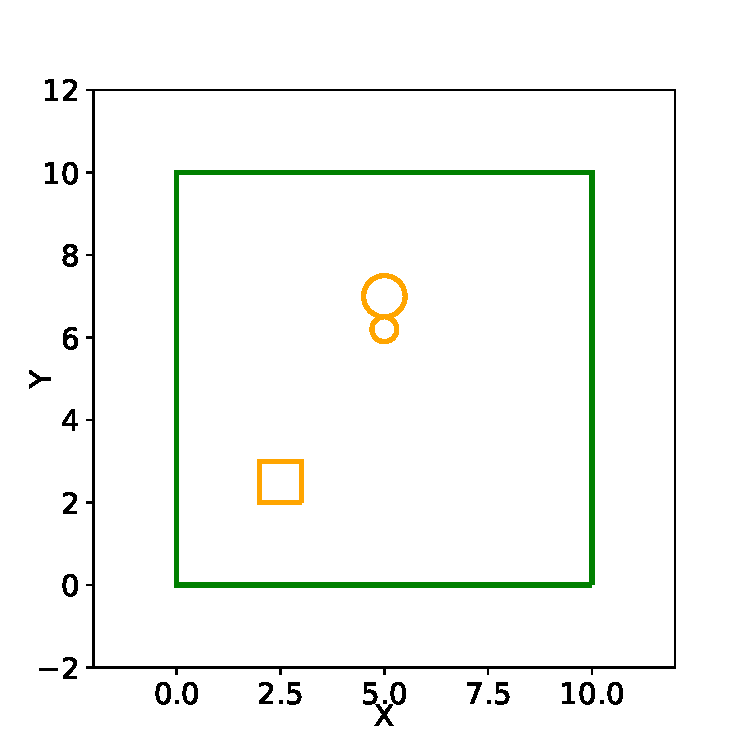
\includegraphics[clip, trim=0cm 0cm 0.0cm 0cm, width=.99\linewidth]{chapter_6_landingsim/figs/map_update_d.pdf}
    \caption{Updated Polygon (UP)\label{fig:ch6_map_update_d}}
  \end{subfigure}
  \caption[Proposed rooftop archival polygon update procedure]{Rooftop archival polygon update with information from onboard sensors. The AP and LP are intersected to create (c). The final polygon to update the rooftop is shown in (d).  }\label{fig:ch6_map_upate}
\end{figure}


\section{Conclusion and Future Work}\label{sec:ch6_conclusions}

This paper presented a real time touchdown point selection algorithm that extracts polygons representing flat surfaces by fusing camera images and LiDAR point cloud data captured by a hovering UAS above the potential unprepared landing site. 
%The greatest inscribed circle within the polygon determines the optimal touchdown position within the surface that maximizes distance to obstacles. 
Our method, Semantic Polylidar3D, combines computer vision using neural networks with computational geometry to create a hybrid algorithm robust to individual sensor/method failure. Evaluation was performed in a high fidelity simulated Unreal Engine city constructed from real world rooftop asset statistics collected from midtown Manhattan, New York. Semantic Polylidar3D showed a greater than 4\% improvement in IoU accuracy for landing site identification compared to a baseline method and took  $\approx$ 30 ms in computation time. The full algorithm, data on Manhattan rooftops, and Unreal Engine world generation scripts are open source and available at \cite{Castagno_Github_UnrealLanding}.

Although our simulated cities model rooftop obstacles accurately, future work is required to build more complete real-world city models that account for building height, textures, streets, parks,  etc. Additionally, our current simulation environment only generates sunny weather image data thus requires extension to more general lighting and weather conditions. As weather conditions worsen, sensors will have degraded performance which will impact the methods presented. Future work should investigate these issues.  Real-world experiments of our touchdown point selection algorithm must also be performed in the future.